% im_foc_ekf_sensorless.tex
% Controllo a orientamento di campo del motore asincrono e stima senza sensore di velocita' con un filtro di Kalman
% esteso: modello, progetto degli anelli, EKF a sei stati (correnti, flusso rotorico, velocita', coppia di carico),
% discretizzazione della predizione, osservabilita', tensione in ingresso e tempo morto, prove in simulazione e
% revisione dell'EKF della libreria (ekf_im_setup, inv_im_param.slx).
% Template pwr-control (AAA_template_latex_settings); numeri e figure: im_foc_ekf_analysis.py (python3, numpy, scipy,
% matplotlib). Compilazione: pdflatex im_foc_ekf_sensorless.tex (tre volte, per i riferimenti).
% Rev. 00 - novembre 2026 - prima emissione
\documentclass[10pt,a4paper]{scrartcl}
\PassOptionsToPackage{main=italian}{babel}   % settings.tex carica babel con [british]: l'italiano diventa la lingua principale
% ===================== PACKAGES =====================
\usepackage[british]{babel}
\usepackage[tmargin=1in, bmargin=1in, lmargin=0.75in, rmargin=0.75in]{geometry}
\usepackage[dvipsnames,table]{xcolor}  % prima di tikz, listings, ecc.

\usepackage{tikz}
\usepackage{graphicx}
\usepackage{pgfplots}
\pgfplotsset{width=12cm, compat=1.9}
\usepackage{setspace}
\usepackage{chemmacros}
\usepackage{chemfig}
\usepackage{esint}
\usepackage{tabularray}
\usepackage{makeidx}
\usepackage{epstopdf}
\usepackage{amssymb}
\usepackage{mathrsfs}
\usepackage{bm}
\usepackage{amsmath}
\usepackage{enumitem}
\usepackage[english]{varioref}
\usepackage{lipsum}
\usepackage{fancyhdr}
\usepackage{float}
\usepackage{empheq}
\usepackage[framemethod=tikz]{mdframed}
\numberwithin{equation}{section}
\usepackage{eso-pic}
\usepackage{calc}
\usepackage{nccmath}
\usepackage{caption}
\usepackage{subcaption}
\usepackage{gensymb}
\usepackage{amsfonts, amsthm, epsfig, epstopdf, titling, url, array}
\usepackage{tabularx}
\usepackage{makecell}
\usepackage{booktabs}
\usepackage{array}
\usepackage{siunitx}
\sisetup{input-digits=0123456789\pi}
\usepackage[symbol]{footmisc}
\usepackage{multicol}
\usepackage{boondox-cal}
\usepackage{blindtext}
\usepackage{changepage}
\usepackage{nomencl}
\usepackage{hyperref}
\usepackage{xurl}
\usepackage{ragged2e}
\usepackage[version=4]{mhchem}  % ← conflitto di opzioni
\usepackage{longtable}
\usepackage{chemformula}
\usetikzlibrary{arrows.meta,positioning,calc}

% ===================== SI UNITS =====================
\DeclareSIUnit\atm{atm}
\DeclareSIUnit{\var}{var}
\DeclareSIUnit{\pu}{p.u.}


% ===================== MATH OPERATORS =====================
\DeclareMathOperator{\rank}{rank}
\DeclareMathOperator{\atantwo}{atan2}
\DeclareMathOperator{\spn}{span}

% ===================== COMMANDS =====================
\newcommand{\abs}[1]{\left|#1\right|}
\newcommand{\sign}{\text{sign}}
\newcommand{\centered}[1]{\begin{tabular}{@{}l@{}} #1 \end{tabular}}

% ===================== COLORS =====================
\definecolor{mycolor1}{rgb}{0.97, 0.97, 0.97}
\definecolor{mycolor2}{rgb}{0.97, 0.97, 0.97}
\definecolor{tableShade}{gray}{0.9}

% ===================== THEOREM ENVIRONMENTS =====================
\theoremstyle{it}
\newtheorem{defn}{Definition}[section]
\newtheorem{assumption}{Assumption}[section]
\newtheorem{thm}{Theorem}[section]
\newtheorem{lemma}{Lemma}[section]
\newtheorem{corollary}{Corollary}[section]
\theoremstyle{definition}
\newtheorem{example}{Example}[section]

% ===================== CUSTOM ENVIRONMENTS =====================
\newenvironment{myitemize_1}{
	\begin{itemize}[topsep=0pt]
		\setlength{\topsep}{2pt}
		\setlength{\itemsep}{2pt}
		\setlength{\parskip}{2pt}
		\setlength{\parsep}{2pt}
	}{\end{itemize}}

\newmdenv[
innerlinewidth=0.5pt,
roundcorner=4pt,
backgroundcolor=mycolor2,
linecolor=mycolor1,
innerleftmargin=6pt,
innerrightmargin=6pt,
innertopmargin=6pt,
innerbottommargin=6pt
]{mybox}

% ===================== TABLE COLUMN TYPES =====================
\newcolumntype{Y}{>{\hsize=2\hsize}X}
\newcolumntype{Z}{>{\centering\arraybackslash\hsize=0.857\hsize}X}

% ===================== SECTION DEPTH =====================
\setcounter{secnumdepth}{3}
\setcounter{tocdepth}{3}

% ===================== PAGE STYLE =====================
\setlength{\headheight}{20pt}
\setlength{\headsep}{20pt}

\pagestyle{fancy}
\fancypagestyle{firstpage}{\rhead{}}
\fancyhead[L]{\slshape\nouppercase{\leftmark}}
\chead{}
\rhead{\includegraphics[height=0.75cm]{../../AAA_template_latex_settings/pwr-control_logo_doc.png}}
\lfoot{\href{http://www.pwr-control.com}{pwr-control.com}}
\cfoot{-\ \thepage\ -}
\rfoot{\textit{}}
\renewcommand{\headrulewidth}{0.4pt}
\renewcommand{\footrulewidth}{0.4pt}


\geometry{
	a4paper,
	top    = 2.5cm,
	bottom = 3.0cm,
	left   = 2.5cm,
	right  = 2.5cm
}

\hypersetup{
	colorlinks = true,
	urlcolor   = blue,
	linkcolor  = black,
	citecolor  = black
}

\pagenumbering{gobble}
% il documento sta tre livelli sotto la radice del repository: percorso del logo di settings.tex corretto qui
\rhead{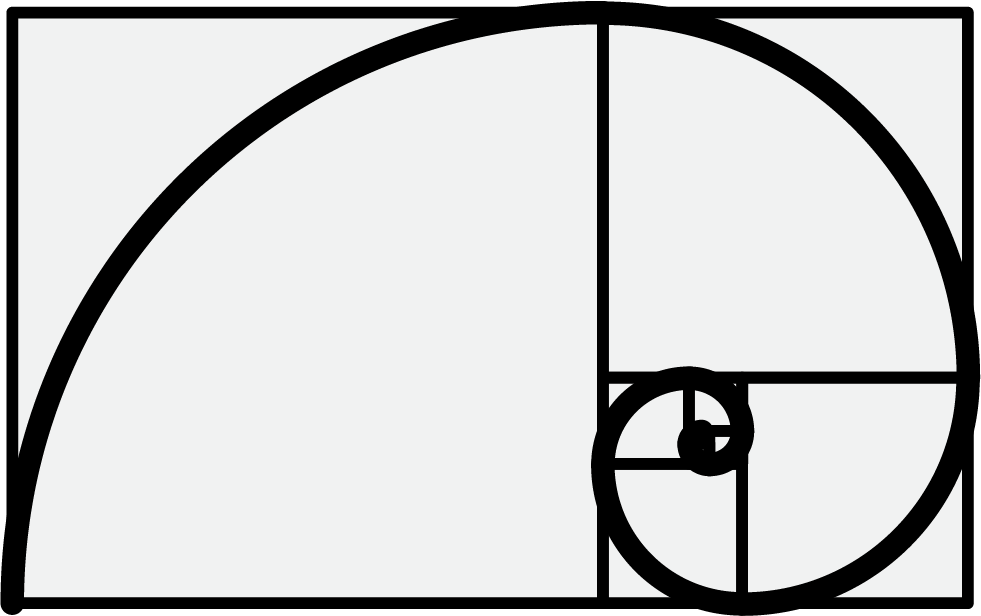
\includegraphics[height=0.75cm]{../../../AAA_template_latex_settings/pwr-control_logo_doc.png}}
\rfoot{\small Rev.~00}
\geometry{left=2.0cm, right=2.0cm}
\newcolumntype{R}[1]{>{\RaggedRight\arraybackslash}p{#1}}

\sisetup{output-decimal-marker={,}, per-mode=symbol, range-phrase={--}, range-units=single, list-final-separator={ e },
         exponent-product=\cdot}
\setlist{nosep}
\setlength{\parindent}{0pt}
\setlength{\parskip}{3pt}
\allowdisplaybreaks

% --- abbreviazioni (non si usano \dd, \abs, \norm, \vec, \grad, \tr, \var, \order, \dv, \wr: occupate da physics/LaTeX) ---
\newcommand{\jj}{\mathrm{j}}
\newcommand{\ee}{\mathrm{e}}
\newcommand{\dif}{\mathrm{d}}
\newcommand{\code}[1]{\texttt{#1}}
\newcommand{\ts}{t_s}
\newcommand{\wb}{\omega_b}
\newcommand{\isv}{\underline{i}_s}
\newcommand{\usv}{\underline{u}_s}
\newcommand{\psv}{\underline{\psi}_r}
\newcommand{\kr}{k_r}
\newcommand{\Lp}{L'}
\newcommand{\Rp}{R'}
\newcommand{\taur}{\tau_r}
\newcommand{\taum}{\tau_m}
\newcommand{\xh}{\hat{x}}
\newcommand{\pu}{\,\mathrm{pu}}
\renewcommand{\Re}{\operatorname{Re}}
\renewcommand{\Im}{\operatorname{Im}}

% =============================================================
%  DATI DEL DOCUMENTO (frontespizio: AAA_template_latex_settings/titlepage.tex)
% =============================================================
\newcommand{\DocCategory}{Nota tecnica}
\newcommand{\DocField}{Elettronica di potenza e sistemi di controllo}
\newcommand{\DocTitle}{%
	{\fontsize{19}{23}\selectfont\bfseries Controllo a orientamento di campo \\[6pt] del motore asincrono} \\[12pt]
	{\fontsize{15}{20}\selectfont\bfseries e stima senza sensore di velocità \\[6pt] con un filtro di Kalman esteso}
}
\newcommand{\DocSubtitle}{La macchina da \SI{261}{kW} dei modelli im\_analysis\_and\_design e inv\_im: \\[6pt] progetto degli anelli, EKF a sei stati, discretizzazione, osservabilità, tempo morto, \\[6pt] prove in simulazione e revisione dell'EKF della libreria}
\newcommand{\DocAuthor}{Davide Bagnara}
\newcommand{\DocRevision}{00}
\newcommand{\DocDate}{Novembre 2026}
\newcommand{\DocAbstract}{%
La nota tratta il controllo a orientamento di campo indiretto del motore asincrono da \SI{261}{kW} (\SI{460}{V}, \SI{60}{Hz}) dei modelli im\_analysis\_and\_design e inv\_im e una sua versione senza sensore basata su un filtro di Kalman esteso (EKF). Il modello è scritto per unità con l'induttore di uscita dell'inverter; gli anelli di corrente (\SI{200}{Hz}), di flusso e di velocità sono progettati con lo zero sul polo e confrontati con i guadagni dei modelli. L'EKF stima correnti, flusso rotorico, velocità e coppia di carico. Il risultato principale riguarda la discretizzazione: con Eulero in avanti a \SI{8}{kHz} il modo del flusso è instabile sopra \num{0.28} pu di velocità e la stima è distorta (\SI{-18}{\degree} di angolo a velocità nominale); la predizione al secondo ordine la rende esatta. Il modello linearizzato perde osservabilità a frequenza di statore nulla. In simulazione il controllo senza sensore tiene la coppia nominale fino al \SI{5}{\percent} della velocità se il tempo morto è compensato entro circa il \SI{10}{\percent}. L'EKF della libreria ha cinque errori di modello o di scala, il più grave sulla riga meccanica (guadagno \num{632} volte troppo alto). Uno script Python riproduce ogni numero e figura.
}
\newcommand{\RevisionHistory}{%
	00 & Novembre 2026 & Prima emissione. & \DocAuthor \\
}
\newcommand{\MetaLabelA}{Repository}
\newcommand{\MetaValueAUrl}{https://github.com/pwr-control/repositories-documentation.git}
\newcommand{\MetaValueALabel}{repositories-documentation.git (research/power\_electronics)}
\newcommand{\MetaLabelB}{Strumenti}
\newcommand{\MetaValueB}{Python 3 (\code{im\_foc\_ekf\_analysis.py}: numpy, scipy, matplotlib)}

\begin{document}
% =============================================================
%  pwr-control LaTeX template - FRONTESPIZIO
%
%  Da richiamare come prima istruzione dopo \begin{document}:
%      \input{../../AAA_template_latex_settings/titlepage}
%
%  Il documento deve definire prima di \begin{document}:
%      \DocCategory   categoria del documento
%      \DocField      area tecnica
%      \DocTitle      titolo (una o due righe)
%      \DocSubtitle   sottotitolo
%      \DocAuthor     autore/i, separati da virgola
%      \DocRevision   numero di revisione corrente (es. 00)
%      \DocDate       data della revisione corrente
%      \DocAbstract   abstract
%      \RevisionHistory  righe della tabella di revisione, nel formato
%                        Rev. & Date & Description & Authors \\
%      \MetaLabelA \MetaValueAUrl \MetaValueALabel
%      \MetaLabelB \MetaValueB
% =============================================================

\providecommand{\DocCategory}{Technical Research Report}
\providecommand{\DocField}{Power Electronics and Control Systems}
\providecommand{\DocSubtitle}{}
\providecommand{\DocRevision}{00}
\providecommand{\DocAbstract}{}
\providecommand{\RevisionHistory}{%
	\DocRevision & \DocDate & First issue. & \DocAuthor \\
}

\titlepage

% ---- Intestazione centrata ----
\begin{center}
	{\Large\scshape \DocCategory}\\[8pt]
	{\large\scshape \DocField}
\end{center}

\vspace{30pt plus 4pt minus 14pt}
\noindent\rule{\linewidth}{0.8pt}

% ---- Titolo ----
\begin{center}
	\DocTitle
\end{center}

\vspace{4pt}
\noindent\rule{\linewidth}{2.2pt}

% ---- Sottotitolo ----
\begin{center}
	\begin{onehalfspace}
		{\large\itshape \DocSubtitle}
	\end{onehalfspace}
\end{center}

% ---- Authors / Revision / Date ----
\vspace{30pt plus 4pt minus 14pt}

\noindent
\begin{minipage}[t]{0.46\linewidth}
	\raggedright
	\textbf{Authors:}\\[2pt]
	\DocAuthor
\end{minipage}%
\hfill
\begin{minipage}[t]{0.22\linewidth}
	\centering
	\textbf{Revision:}\\[2pt]
	\DocRevision
\end{minipage}%
\hfill
\begin{minipage}[t]{0.30\linewidth}
	\raggedleft
	\textbf{Date:}\\[2pt]
	\DocDate
\end{minipage}

\vspace{10pt}
\noindent\rule{\linewidth}{0.8pt}

% ---- Abstract ----
\vspace{24pt plus 4pt minus 12pt}

\begin{center}
	\begin{minipage}{0.88\linewidth}
		\footnotesize
		\begin{onehalfspace}
			\textbf{Abstract:} \DocAbstract
		\end{onehalfspace}
	\end{minipage}
\end{center}

\vfill

% ---- Revision history ----
\begin{center}
	\begin{minipage}{0.96\linewidth}
		\centering
		{\footnotesize\scshape Revision history}\\[6pt]
		{\footnotesize
			\begin{tabular}{@{}cl>{\raggedright\arraybackslash}p{0.36\linewidth}>{\raggedright\arraybackslash}p{0.28\linewidth}@{}}
				\toprule
				\textbf{Rev.} & \textbf{Date} & \textbf{Description} & \textbf{Authors} \\
				\midrule
				\RevisionHistory
				\bottomrule
			\end{tabular}}
	\end{minipage}
\end{center}

\vspace{18pt plus 4pt minus 10pt}

% ---- Metadati in fondo ----
\noindent
\begin{tabular}{@{} r @{\quad} l @{}}
	\textsc{\MetaLabelA:} & {\href{\MetaValueAUrl}{\MetaValueALabel}} \\[3pt]
	\textsc{\MetaLabelB:} & {\MetaValueB}       \\[3pt]
\end{tabular}

% =============================================================
%  Fine frontespizio
% =============================================================
\newpage
\pagenumbering{arabic}
\setcounter{page}{1}

\tableofcontents
\newpage
\begin{onehalfspace}

% =====================================================================================================
\section{Scopo, modelli di riferimento e dati}
\label{sec:scopo}

La nota descrive il controllo a orientamento di campo (FOC) del motore asincrono e la sua estensione senza sensore di velocità con un filtro di Kalman esteso (EKF). Si riferisce a due modelli del repository modelization-and-control, entrambi in \path{foundations_of_power_electronics}:
\begin{itemize}
\item \code{im\_analysis\_and\_design}: FOC indiretto con encoder, osservatore di flusso a modello di corrente, inverter mediato o a interruttori ideali; i guadagni e le criticità del modello sono nella revisione allegata alla PR~\#20 di quel repository;
\item \code{inv\_im}: la stessa macchina su inverter con il blocco \code{ekf/extended\_kalman\_observer} di \code{inv\_im\_param.slx}, configurato dalla classe \code{ekf\_im\_setup} della libreria. Lo switch encoder/sensorless del modello ha lo \code{Step} \code{time\_use\_im\_ekf} commentato, quindi il controllo usa sempre l'encoder e l'EKF gira in parallelo senza entrare nell'anello.
\end{itemize}

Il percorso è: modello e per unità (Sez.~\ref{sec:modello}), FOC con encoder e progetto degli anelli (Sez.~\ref{sec:foc}), metodi senza sensore (Sez.~\ref{sec:panoramica}), EKF (Sez.~\ref{sec:ekf}), prove in simulazione (Sez.~\ref{sec:prove}), revisione dell'EKF della libreria (Sez.~\ref{sec:libreria}) e raccomandazioni (Sez.~\ref{sec:raccomandazioni}). Ogni numero è calcolato dallo script \code{im\_foc\_ekf\_analysis.py}, che riproduce anche le figure. I dati sono in Tab.~\ref{tab:dati}; i parametri del circuito equivalente sono quelli che \code{im\_setup} ricava dalla targa e dalle prove a vuoto e a rotore bloccato.

\begin{table}[H]
\centering\small
\begin{tabular}{@{}R{5.2cm}R{10.3cm}@{}}
\toprule
\textbf{Voce} & \textbf{Valore} \\
\midrule
Macchina & ABB M3BP 355MLB 6: \SI{261}{kW}, \SI{460}{V}, \SI{411}{A}, \SI{60}{Hz}, sei poli ($p = 3$), \SI{1195}{rpm}, $J = \SI{5}{kg.m^2}$ \\
Circuito equivalente (\code{im\_setup}) & $R_s = \SI{2.00}{m\ohm}$, $R_r = \SI{2.740}{m\ohm}$, $L_s = L_r = \SI{3.9138}{mH}$, $L_m = \SI{3.7633}{mH}$, $\sigma L_s = \SI{0.2950}{mH}$, $\taur = L_r/R_r = \SI{1.428}{s}$ \\
Carico & attrito viscoso pari a $0.75\,T_{nom}$ alla velocità sincrona (\code{load\_friction} di \code{im\_setup}) più una coppia esterna \\
Inverter & due livelli, \SI{4}{kHz} con doppio aggiornamento: periodo di controllo $\ts = \SI{125}{\micro s}$; tempo morto \SI{3}{\micro s} (\code{param.inv.pwm.dead\_time} di inv\_im) \\
Induttore di uscita & $L_{Fi} = \SI{230}{\micro H}$, $R_{Fi} = \SI{1.81}{m\ohm}$ (set \SI{690}{V} della libreria) \\
DC link & \SI{1200}{V} (batteria); unità di tensione di controllo $u_{dc}/\sqrt3 = \SI{692.8}{V}$ di picco \\
Misura di corrente & \SI{12}{bit} su $\pm\SI{1049.8}{A}$ (passo \SI{0.51}{A}), più \SI{1}{A} efficace di rumore bianco per fase \\
\bottomrule
\end{tabular}
\caption{Dati della macchina, dell'inverter e della misura usati nella nota.}
\label{tab:dati}
\end{table}

% =====================================================================================================
\section{Modello della macchina}
\label{sec:modello}

\subsection{Equazioni nel riferimento stazionario}
\label{sec:equazioni}

Con i vettori spaziali a conservazione di ampiezza ($\underline{x} = \tfrac23(x_a + x_b\,\ee^{\jj 2\pi/3} + x_c\,\ee^{-\jj 2\pi/3}) = x_\alpha + \jj x_\beta$) e come stati la corrente di statore $\isv$ e il flusso rotorico $\psv$, la macchina nel riferimento stazionario è
\begin{align}
\Lp\,\frac{\dif \isv}{\dif t} &= \usv - \Rp\,\isv + \kr\left(\frac{1}{\taur} - \jj\omega\right)\psv, \label{eq:corrente}\\
\frac{\dif \psv}{\dif t} &= \frac{L_m\,\isv - \psv}{\taur} + \jj\omega\,\psv, \label{eq:flusso}\\
T &= \frac32\,p\,\kr\,\Im\!\left(\psv^{*}\,\isv\right), \qquad J\,\frac{\dif\omega_m}{\dif t} = T - T_L, \label{eq:meccanica}
\end{align}
con $\kr = L_m/L_r$, $\omega = p\,\omega_m$ pulsazione elettrica del rotore, $\taur = L_r/R_r$. L'inverter vede la macchina attraverso l'induttore di uscita, quindi l'induttanza e la resistenza della \eqref{eq:corrente} sono quelle totali:
\begin{equation}
\Lp = \sigma L_s + L_{Fi} = \SI{0.525}{mH}, \qquad \Rp = R_s + R_{Fi} + \kr^2 R_r = \SI{6.34}{m\ohm}.
\label{eq:lpr}
\end{equation}
L'induttore aumenta l'induttanza transitoria di \num{1.78} volte: un EKF che usa $\sigma L_s$ della sola macchina sbaglia la dinamica della corrente di altrettanto (Sez.~\ref{sec:libreria}).

\subsection{Per unità}
\label{sec:pu}

Le basi sono quelle di \code{im\_setup}: $u_b = \sqrt2\,U_n/\sqrt3 = \SI{375.6}{V}$, $i_b = \sqrt2\,I_n = \SI{581.2}{A}$, $\wb = 2\pi\cdot\SI{60}{Hz}$, $Z_b = u_b/i_b = \SI{0.6462}{\ohm}$, $L_b = Z_b/\wb = \SI{1.7141}{mH}$, $\psi_b = u_b/\wb = \SI{0.9963}{Wb}$. La base di coppia naturale è $T_b = \tfrac32\,p\,\psi_b\,i_b = \SI{2606}{N.m}$: con questa base la coppia in pu è $T = \kr\,\Im(\psv^{*}\isv)$ senza altri fattori. La coppia \code{torque\_nom} di \code{im\_setup} (\SI{2186}{N.m}, potenza nominale divisa per il rendimento e per la velocità sincrona) non è una base coerente con le altre ed è diversa anche dalla coppia all'albero nel punto nominale (\SI{2086}{N.m}); la coppia nominale vale \num{0.84} pu di $T_b$.

Con il tempo in secondi e le grandezze in pu le equazioni diventano
\begin{align}
\frac{\dif \isv}{\dif t} &= \wb\left[-\gamma\,\isv + \beta\,(\alpha - \jj\omega)\,\psv + \frac{\usv}{\sigma}\right], \label{eq:correntepu}\\
\frac{\dif \psv}{\dif t} &= \wb\left[\alpha\,L_m\,\isv - \alpha\,\psv + \jj\omega\,\psv\right], \label{eq:flussopu}\\
\frac{\dif \omega}{\dif t} &= \frac{\kr\,\Im(\psv^{*}\isv) - T_L}{\taum}, \qquad \taum = \frac{J\,\omega_{mb}}{T_b} = \SI{0.2411}{s}, \label{eq:meccanicapu}
\end{align}
con $\omega_{mb} = \wb/p$ e i coefficienti normalizzati di Tab.~\ref{tab:coeff}: $\sigma$ è l'induttanza transitoria in pu, $\alpha = R_r/L_r = 1/(\wb\taur)$, $\beta = L_m/(\sigma L_r)$ e $\gamma = R_s/\sigma + \alpha\beta L_m$. Con l'induttore di uscita si usano $\sigma_t$ e $R_{s,t}$ al posto di $\sigma$ e $R_s$.

\begin{table}[H]
\centering\small
\begin{tabular}{@{}lcccccccc@{}}
\toprule
 & $L_s$, $L_r$ & $L_m$ & $\sigma$ & $R_s$ & $R_r$ & $\alpha$ & $\beta$ & $\gamma$ \\
\midrule
macchina & \num{2.2833} & \num{2.1956} & \num{0.17212} & \num{0.00310} & \num{0.00424} & \num{0.001857} & \num{5.586} & \num{0.04076} \\
con $L_{Fi}$, $R_{Fi}$ & & & \num{0.30631} & \num{0.00589} & & & \num{3.139} & \num{0.03203} \\
\bottomrule
\end{tabular}
\caption{Coefficienti normalizzati (pu); nella seconda riga quelli che cambiano con l'induttore di uscita. La costante meccanica nella base naturale è $\taum = \SI{0.2411}{s}$; la libreria usa invece $J_{m,norm} = \tfrac12 J\omega_{mb}/T_{nom} = \SI{0.1437}{s}$ (Sez.~\ref{sec:libreria}).}
\label{tab:coeff}
\end{table}

\subsection{Coordinate di flusso rotorico}
\label{sec:coordinate}

Nel riferimento $xy$ con l'asse $x$ sul flusso rotorico ($\psv = \psi\,\ee^{\jj\theta_\psi}$, $\psi$ reale) la \eqref{eq:flusso} si separa in modulo e pulsazione:
\begin{equation}
\taur\,\frac{\dif\psi}{\dif t} + \psi = L_m\,i_{sx}, \qquad \omega_\psi = \frac{\dif\theta_\psi}{\dif t} = \omega + \frac{L_m\,i_{sy}}{\taur\,\psi}, \qquad T = \frac32\,p\,\kr\,\psi\,i_{sy}.
\label{eq:foc}
\end{equation}
Il flusso è governato dalla sola $i_{sx}$ con la costante di tempo rotorica, la coppia è proporzionale a $\psi\,i_{sy}$ e la pulsazione di scorrimento $\omega_{sl} = L_m i_{sy}/(\taur\psi)$ è fissata dalla coppia. A regime $\psi = L_m i_{sx}$ e $\omega_{sl} = i_{sy}/(\taur i_{sx})$: con flusso 1 pu e coppia 1 pu lo scorrimento vale \num{0.0042} pu, cioè \SI{0.25}{Hz}. Con $\taur = \SI{1.43}{s}$ il flusso è molto lento da costruire e la macchina va magnetizzata prima di chiedere coppia (Sez.~\ref{sec:anelloflusso}).

% =====================================================================================================
\section{Controllo a orientamento di campo}
\label{sec:foc}

\subsection{Struttura}
\label{sec:struttura}

La struttura è quella di Fig.~\ref{fig:schema}. L'anello di velocità dà il riferimento di coppia, diviso per $\kr\hat\psi$ per ottenere $i_{sy,ref}$. L'anello di flusso dà $i_{sx,ref}$, con un feed-forward del valore di regime. Due PI di corrente in $xy$, con il disaccoppiamento in avanti, danno la tensione, che è ruotata nel riferimento stazionario con l'angolo anticipato di $1.5\,\ts\,\omega_\psi$ e mandata alla modulazione vettoriale. Angolo, modulo del flusso e velocità vengono dall'osservatore a modello di corrente con l'encoder (Sez.~\ref{sec:osservatore}) oppure dall'EKF (Sez.~\ref{sec:ekf}).

\begin{figure}[htb]
\centering
\begin{tikzpicture}[>=Latex, font=\footnotesize,
  blk/.style={draw, minimum height=7mm, minimum width=10mm, inner sep=3pt, align=center, fill=gray!8},
  sum/.style={draw, circle, minimum size=4mm, inner sep=0pt}]
\node (wref) at (0,0) {$\omega_{ref}$};
\node[sum] (s1) at (1.0,0) {};
\node[blk] (piw) at (2.2,0) {PI$_\omega$};
\node[blk] (div) at (4.3,0) {$\dfrac{T_{ref}}{\kr\hat\psi}$};
\node (psiref) at (0,-1.6) {$\psi_{ref}$};
\node[sum] (s2) at (1.6,-1.6) {};
\node[blk] (pipsi) at (3.0,-1.6) {PI$_\psi$ + FF};
\node[sum] (s3) at (6.1,-0.8) {};
\node[blk] (pii) at (7.5,-0.8) {PI$_i$ +\\disacc.};
\node[blk] (rot) at (10.3,-0.8) {$\ee^{\jj(\hat\theta_\psi + 1.5\ts\omega_\psi)}$};
\node[sum] (s4) at (12.4,-0.8) {};
\node[blk] (svm) at (13.75,-0.8) {SVM +\\inverter};
\node[blk] (mot) at (15.75,-0.8) {$L_{Fi}$ +\\motore};
\node[blk] (dtc) at (12.4,0.75) {compensazione\\tempo morto};
\node[blk] (cla) at (15.75,-2.6) {Clarke};
\node[blk] (irot) at (7.5,-2.6) {$\ee^{-\jj\hat\theta_\psi}$};
\node[blk] (ekf) at (7.5,-4.2) {EKF (o osservatore + encoder)};
\node[blk] (dly) at (11.85,-4.2) {$z^{-1}$};
\draw[->] (wref) -- (s1);
\draw[->] (s1) -- (piw);
\draw[->] (piw) -- node[above]{$T_{ref}$} (div);
\draw[->] (div) -| node[pos=0.3, above]{$i_{sy,ref}$} (s3);
\draw[->] (psiref) -- (s2);
\draw[->] (s2) -- (pipsi);
\draw[->] (pipsi) -| node[pos=0.3, below]{$i_{sx,ref}$} (s3);
\draw[->] (s3) -- (pii);
\draw[->] (pii) -- node[above]{$u_{xy}$} (rot);
\draw[->] (rot) -- (s4);
\draw[->] (dtc) -- (s4);
\draw[->] (s4) -- (svm);
\draw[->] (svm) -- (mot);
\draw[->] (mot) -- node[right]{$i_{abc}$} (cla);
\draw[->] (cla) -- node[above]{$\underline{i}_{s}$} (irot);
\draw[->] (irot) -| node[pos=0.8, right]{$i_{xy}$} (s3);
\coordinate (tap) at (11.85,-0.8);
\fill (tap) circle (1.3pt);
\draw[->] (tap) -- node[pos=0.82, right]{$\usv$} (dly);
\draw[->] (dly) -- (ekf);
\draw[->] (cla.south) -- (15.75,-4.9) -| node[pos=0.25, below]{$\underline{i}_{s}$} (ekf.south);
\draw[->] (ekf.west) -| node[pos=0.92, right]{$\hat\psi$} (s2.south);
\draw[->] (ekf.west) -| node[pos=0.95, left]{$\hat\omega$} (s1.south);
\node[font=\scriptsize, align=left, anchor=west] at (2.0,-3.75) {$\hat\theta_\psi$ alle rotazioni, $\hat\psi$ al divisore};
\end{tikzpicture}
\caption{Struttura del controllo. La compensazione del tempo morto si somma al comando della modulazione; l'EKF riceve la tensione del regolatore di corrente (senza la compensazione) applicata nell'ultimo intervallo e la corrente campionata. Nel funzionamento con encoder angolo e flusso vengono dall'osservatore a modello di corrente (Sez.~\ref{sec:osservatore}).}
\label{fig:schema}
\end{figure}

\subsection{Osservatore di flusso con encoder}
\label{sec:osservatore}

Nel FOC indiretto con encoder il flusso si ottiene integrando la \eqref{eq:flusso} nel riferimento del rotore, dove il termine $\jj\omega\psv$ sparisce:
\begin{equation}
\psv^{(r)}[k+1] = \psv^{(r)}[k] + \ts\,\wb\,\alpha\left(L_m\,\isv[k]\,\ee^{-\jj\theta_{enc}[k]} - \psv^{(r)}[k]\right), \qquad \psv = \psv^{(r)}\,\ee^{\jj\theta_{enc}}.
\label{eq:osservatore}
\end{equation}
È il modello di corrente: non usa la tensione, quindi funziona fino a velocità nulla, ma dipende da $\taur$ e da $L_m$. Un errore su $\taur$ (la resistenza rotorica varia del \SIrange{30}{40}{\percent} con la temperatura) sposta l'angolo stimato in modo proporzionale allo scorrimento, quindi soprattutto a coppia elevata. Nel riferimento del rotore la \eqref{eq:osservatore} è un filtro del primo ordine stabile con Eulero, perché il polo $-\alpha\wb$ è reale; la rotazione è esatta perché usa l'angolo dell'encoder.

\subsection{Anello di corrente}
\label{sec:anellocorrente}

Nel riferimento $xy$, con il flusso quasi costante alla scala dei tempi della corrente, la \eqref{eq:corrente} è
\begin{equation}
\Lp\,\frac{\dif\underline{i}_{xy}}{\dif t} = \underline{u}_{xy} - \Rp\,\underline{i}_{xy} - \jj\omega_\psi\left(\Lp\,\underline{i}_{xy} + \kr\,\psi\right) + \kr\,\psi\left(\frac{1}{\taur} + \jj\omega_{sl}\right).
\label{eq:correntexy}
\end{equation}
Il disaccoppiamento in avanti $\underline{u}_{ff} = \jj\omega_\psi(\Lp\,\underline{i}_{xy} + \kr\psi)$ toglie i termini incrociati e la forza controelettromotrice; l'ultimo termine è lento (vale $\kr^2 R_r\,\underline{i}_{xy}$ a regime) e lo recupera l'integrale. Resta l'impianto $1/(\Rp + s\Lp)$ con il ritardo di $1.5\,\ts$ (un periodo di calcolo più mezzo periodo di mantenimento della modulazione). Il PI con lo zero sul polo elettrico, $k_i/k_p = \Rp/\Lp$, dà un anello aperto $\omega_c/s$ con
\begin{equation}
k_p = \omega_c\,\Lp, \qquad k_i = \omega_c\,\Rp, \qquad \text{margine di fase} = \SI{90}{\degree} - \omega_c\cdot 1.5\,\ts.
\label{eq:imc}
\end{equation}
È il progetto a modello interno di \cite{harnefors1998}. Con $f_c = \SI{200}{Hz}$ (un ventesimo della frequenza di Nyquist) i guadagni nell'unità di controllo ($u_{dc}/\sqrt3$ per $i_b$) sono $k_p = \num{0.554}$ e $k_i = \SI{6.68}{s^{-1}}$, con margine di fase di \SI{76}{\degree}. La costante elettrica è $\Lp/\Rp = \SI{82.8}{ms}$. I guadagni del modello im\_analysis\_and\_design ($k_p = \num{0.25}$, $k_i = \SI{18}{s^{-1}}$) danno \SI{91}{Hz} e \SI{78}{\degree} (Tab.~\ref{tab:guadagni}, Fig.~\ref{fig:anelli}).

La tensione è limitata in modulo a 1 (il cerchio inscritto dell'esagono della modulazione vettoriale) e l'integrale si ferma quando il limite è attivo. I guadagni in pu dell'unità di controllo valgono per $u_{dc} = \SI{1200}{V}$: senza feed-forward della tensione di batteria (l'ingresso udc della modulazione nei modelli è la costante 1) il guadagno d'anello segue la $u_{dc}$ reale. Dividere la tensione di riferimento per la $u_{dc}$ misurata in pu toglie questa dipendenza.

\subsection{Anello di flusso, magnetizzazione e deflussaggio}
\label{sec:anelloflusso}

L'impianto è $\psi/(L_m i_{sx}) = 1/(1 + s\taur)$. Il regolatore proposto è un feed-forward del valore di regime più un PI con lo zero sul polo rotorico:
\begin{equation}
L_m\,i_{sx,ref} = \psi_{ref} + k_{p\psi}\,(\psi_{ref} - \hat\psi) + k_{i\psi}\int(\psi_{ref} - \hat\psi)\,\dif t, \qquad k_{i\psi} = \frac{k_{p\psi}}{\taur},
\label{eq:pipsi}
\end{equation}
con l'integrale fermo quando $i_{sx,ref}$ è al limite. Con $k_{p\psi} = 6$ l'anello aperto è $k_{p\psi}/(s\taur)$: attraversamento a \SI{0.67}{Hz} con \SI{90}{\degree} di margine e costante di tempo in anello chiuso $\taur/k_{p\psi} = \SI{0.238}{s}$. Il PI del modello ($k_p = 2$, $k_i = \SI{20}{s^{-1}}$, anti-windup a ricalcolo) ha \SI{31}{\degree} di margine e sovraelonga all'uscita dalla saturazione.

La magnetizzazione è limitata dalla corrente: con $i_{sx} \le \num{0.8}$ pu il flusso tende a $\num{0.8}\,L_m = \num{1.76}$ pu con costante $\taur$ e arriva a circa \num{0.88} pu dopo \SI{1}{s}. La rampa di velocità deve partire dopo la magnetizzazione; il riferimento di coppia diviso per $\hat\psi$ (con un minimo, qui \num{0.3} pu) compensa il flusso non ancora pieno con più corrente $i_{sy}$. Durante la magnetizzazione in continua la velocità non è osservabile (Sez.~\ref{sec:osservabilita}): l'EKF tiene $\hat\omega = \hat T_L = 0$ finché la rampa non parte.

Il deflussaggio sopra la velocità base va legato alla tensione: un anello lento sul modulo della tensione di controllo che riduce $\psi_{ref}$ quando supera \numrange{0.85}{0.9}. La legge $1/\omega^2$ dei modelli parte da \num{1} pu anche se lì la tensione è \num{0.61} e riduce il flusso più del necessario (la legge a tensione costante è $1/\omega$).

\subsection{Anello di velocità}
\label{sec:anellovelocita}

L'uscita del PI di velocità è la coppia (non $i_{sy}$): il guadagno d'anello non dipende dal flusso, e quindi resta lo stesso in magnetizzazione e in deflussaggio. L'impianto è $\omega/T = 1/(\taum s + b)$, con $b$ il coefficiente d'attrito in pu (polo a \SI{2.61}{rad/s}), in serie all'anello di corrente chiuso. Con
\begin{equation}
k_{p\omega} = \omega_{c\omega}\,\taum, \qquad k_{i\omega} = k_{p\omega}\,\frac{\omega_{c\omega}}{4}
\label{eq:piw}
\end{equation}
e $f_{c\omega} = \SI{3}{Hz}$ si ha $k_{p\omega} = \num{4.54}$ e $k_{i\omega} = \SI{21.4}{s^{-1}}$ (coppia in pu di $T_b$ per pu di velocità): attraversamento a \SI{3.06}{Hz} con \SI{83}{\degree} di margine. Il PI del modello ha uscita $i_{sy}$ ($k_p = \num{2.5}$, $k_i = \SI{18}{s^{-1}}$): \SI{1.83}{Hz} e \SI{70}{\degree} a flusso nominale, con banda che scala con il flusso.

La banda dell'anello di velocità fissa anche la caduta di velocità a un gradino di carico, dell'ordine di $\Delta T/k_{p\omega}$: un gradino di \num{0.6} pu dà circa \num{0.13} pu di caduta. Al \SI{5}{\percent} della velocità un gradino così porta la macchina oltre lo zero di velocità, cioè nella zona dove la stima senza sensore è più debole (Sez.~\ref{sec:prove}).

\begin{table}[H]
\centering\small
\begin{tabular}{@{}lcccc@{}}
\toprule
Anello & Guadagni del modello & Banda, margine & Guadagni proposti & Banda, margine \\
\midrule
corrente & $k_p = \num{0.25}$, $k_i = \SI{18}{s^{-1}}$ & \SI{91}{Hz}, \SI{78}{\degree} & $k_p = \num{0.554}$, $k_i = \SI{6.68}{s^{-1}}$ & \SI{200}{Hz}, \SI{76}{\degree} \\
flusso & $k_p = 2$, $k_i = \SI{20}{s^{-1}}$ & \SI{0.61}{Hz}, \SI{31}{\degree} & $k_p = 6$, $k_i = \SI{4.20}{s^{-1}}$ + FF & \SI{0.67}{Hz}, \SI{90}{\degree} \\
velocità & $k_p = \num{2.5}$, $k_i = \SI{18}{s^{-1}}$ (uscita $i_{sy}$) & \SI{1.83}{Hz}, \SI{70}{\degree} & $k_p = \num{4.54}$, $k_i = \SI{21.4}{s^{-1}}$ (uscita $T$) & \SI{3.06}{Hz}, \SI{83}{\degree} \\
\bottomrule
\end{tabular}
\caption{Guadagni degli anelli: modello im\_analysis\_and\_design e proposta di questa nota (corrente nell'unità $u_{dc}/\sqrt3$ per $i_b$; flusso e velocità in pu). Gli anelli sono quelli di Fig.~\ref{fig:anelli}.}
\label{tab:guadagni}
\end{table}

\begin{figure}[htb]
\centering
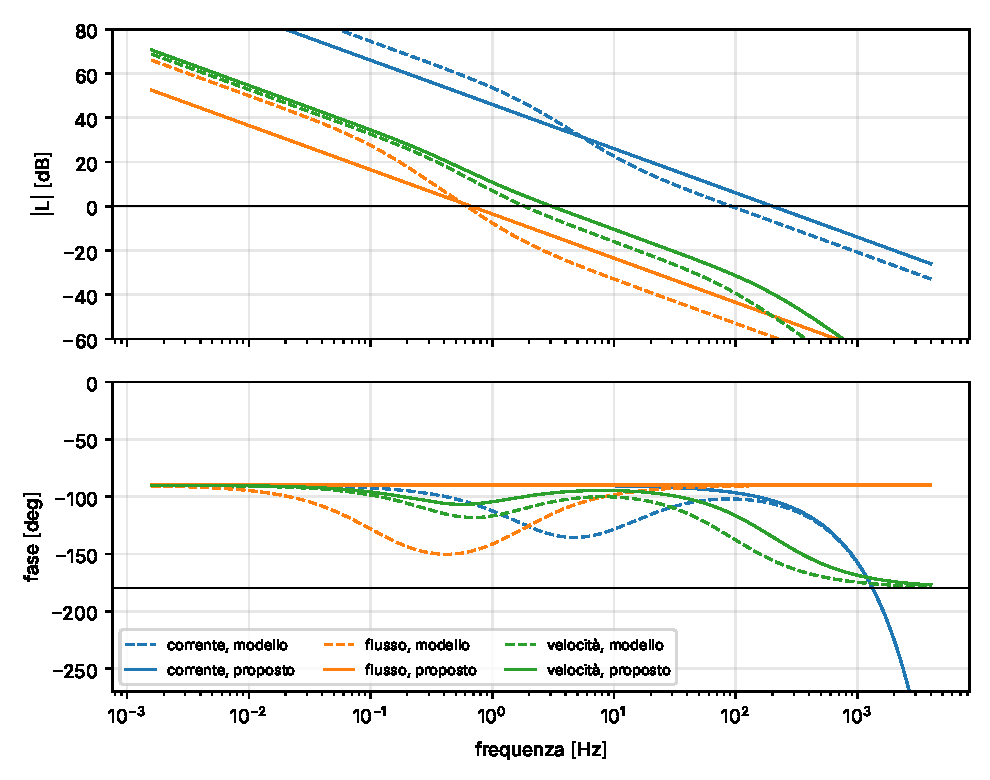
\includegraphics[width=0.85\linewidth]{figures/fig_foc_loops.pdf}
\caption{Anelli aperti di corrente, flusso e velocità con i guadagni del modello (tratteggio) e con quelli proposti (linea continua), con il ritardo di $1.5\,\ts$ e il PI discreto.}
\label{fig:anelli}
\end{figure}

% =====================================================================================================
\section{Stima senza sensore: panoramica}
\label{sec:panoramica}

Senza encoder il controllo deve stimare l'angolo del flusso rotorico (per le rotazioni), il modulo del flusso (per l'anello di flusso e la divisione della coppia) e la velocità (per l'anello di velocità). I metodi basati sul modello usano le sole tensioni e correnti di statore \cite{holtz2002, vas1998}:
\begin{itemize}
\item \emph{modello di tensione in anello aperto}: integra $\usv - R_s\isv$; semplice, ma l'integrazione deriva per gli offset e l'errore su $R_s$ domina a bassa velocità;
\item \emph{MRAS} \cite{schauder1992}: confronta un modello di tensione e uno di corrente del flusso e adatta la velocità; eredita i limiti del modello di tensione;
\item \emph{osservatori adattativi di ordine pieno} \cite{kubota1993}: osservatore di Luenberger su correnti e flusso con legge di adattamento della velocità; richiedono un progetto dei guadagni attento in rigenerazione a bassa velocità \cite{hinkkanen2004};
\item \emph{filtro di Kalman esteso} \cite{kim1994, barut2007}: stima insieme correnti, flusso, velocità e, se serve, coppia di carico; i guadagni seguono dalle covarianze dei disturbi e del rumore di misura, e la coppia di carico stimata riduce il ritardo della stima di velocità nei transitori. Il costo è il calcolo (matrici $6\times6$ a ogni passo) e la taratura di $Q$ e $R$;
\item \emph{iniezione di segnale}: sfrutta salienze; nel motore asincrono ci sono solo quelle da saturazione e da cave, deboli e dipendenti dal carico; è l'unica via per lavorare a lungo a frequenza nulla.
\end{itemize}

Tutti i metodi basati sul modello hanno lo stesso limite di fondo: a frequenza di statore nulla la macchina non è osservabile dalle grandezze di statore (Sez.~\ref{sec:osservabilita}). Il resto della nota sviluppa l'EKF, che è la scelta del modello inv\_im e quella richiesta.

% =====================================================================================================
\section{Filtro di Kalman esteso}
\label{sec:ekf}

\subsection{Modello di stato}
\label{sec:stato}

Lo stato è $x = [i_\alpha,\ i_\beta,\ \psi_\alpha,\ \psi_\beta,\ \omega,\ T_L]^T$ in pu, l'ingresso è la tensione $u = [u_\alpha,\ u_\beta]^T$ in pu di $u_b$, l'uscita misurata è la corrente, $y = C x = [i_\alpha,\ i_\beta]^T$. Le equazioni sono le \eqref{eq:correntepu}--\eqref{eq:meccanicapu} con $\sigma_t$ e $R_{s,t}$ e la coppia di carico come passeggiata aleatoria:
\begin{equation}
\dot x = f(x,u) + w, \qquad f(x,u) =
\begin{bmatrix}
\wb\left(-\gamma\,i_\alpha + \beta\alpha\,\psi_\alpha + \beta\,\omega\,\psi_\beta + u_\alpha/\sigma\right)\\
\wb\left(-\gamma\,i_\beta + \beta\alpha\,\psi_\beta - \beta\,\omega\,\psi_\alpha + u_\beta/\sigma\right)\\
\wb\left(\alpha L_m\,i_\alpha - \alpha\,\psi_\alpha - \omega\,\psi_\beta\right)\\
\wb\left(\alpha L_m\,i_\beta - \alpha\,\psi_\beta + \omega\,\psi_\alpha\right)\\
\left(\kr(\psi_\alpha i_\beta - \psi_\beta i_\alpha) - T_L\right)/\taum\\
0
\end{bmatrix},
\label{eq:f}
\end{equation}
$y_k = C x_k + v_k$, con $w$ e $v$ rumori bianchi di covarianza $Q$ (per passo) e $R$. La coppia di carico stimata comprende l'attrito: è la coppia che manca al bilancio meccanico. La Jacobiana $A(x) = \partial f/\partial x$ è in Appendice~\ref{app:matrici}. Con il modello meccanico la velocità non è una semplice passeggiata aleatoria: segue la coppia elettromagnetica stimata, e la stima di $T_L$ assorbe il carico. È la differenza principale rispetto al modello a cinque stati (velocità come passeggiata aleatoria), che deve lasciare a $Q_\omega$ il compito di seguire le accelerazioni e quindi passa più rumore alla velocità.

\subsection{Discretizzazione della predizione}
\label{sec:discretizzazione}

La predizione con Eulero in avanti, $\xh_{k+1|k} = \xh_k + \ts f(\xh_k, u_k)$ e $\Phi_k = I + \ts A(\xh_k)$, è la scelta più comune ed è quella dell'EKF della libreria. Qui non va bene. Il modo del flusso ha nel continuo l'autovalore $\lambda \approx \wb(-\alpha + \jj\omega)$; Eulero lo porta in $1 + \ts\lambda$, il cui modulo è
\begin{equation}
\left|1 + \ts\lambda\right| \approx 1 - \alpha\,\wb\ts + \frac{(\omega\,\wb\ts)^2}{2}.
\label{eq:eulero}
\end{equation}
Lo smorzamento rotorico per passo è $\alpha\wb\ts = \num{8.75e-5}$, mentre il termine di rotazione a velocità nominale vale $(\wb\ts)^2/2 = \num{1.11e-3}$, tredici volte di più: il modo del flusso discreto è instabile sopra
\begin{equation}
\omega > \sqrt{\frac{2\alpha}{\wb\ts}} = \num{0.281}\pu .
\label{eq:wcrit}
\end{equation}
Il fenomeno è lo stesso del termine risonante discretizzato con Eulero nella nota sul grid-forming \cite{pwrgfm}: con una costante di tempo lunga ($\taur = \SI{1.43}{s}$) basta una rotazione di \SI{2.7}{\degree} per passo per superare lo smorzamento. Sul modello elettrico completo ($4\times4$) a velocità e coppia nominali il massimo modulo degli autovalori vale \num{1.000419} con Eulero contro \num{0.999310} esatto. Il filtro corregge la divergenza con le innovazioni di corrente, ma lo fa spostando lo stato: in simulazione (Sez.~\ref{sec:r1}) la stima dell'angolo a velocità nominale ha \SI{-18.35}{\degree} di errore e la velocità \num{-0.035} pu.

La predizione di Taylor al secondo ordine risolve il problema con poco calcolo in più:
\begin{equation}
\xh_{k+1|k} = \xh_k + \ts f(\xh_k,u_k) + \frac{\ts^2}{2}\,A(\xh_k)\,f(\xh_k,u_k), \qquad \Phi_k = I + \ts A(\xh_k) + \frac{\ts^2}{2}A(\xh_k)^2.
\label{eq:taylor2}
\end{equation}
Il massimo modulo degli autovalori diventa \num{0.999289}, praticamente quello esatto, e l'errore della \eqref{eq:eulero} scende all'ordine $(\omega\wb\ts)^4/8 = \num{6e-7}$ per passo. In simulazione serve il secondo ordine nella predizione dello stato; per la covarianza basta $\Phi_k = I + \ts A(\xh_k)$ (stessi risultati in R1 e R2), il che evita il prodotto $A^2$. In alternativa si può ruotare il flusso in modo esatto o integrare con due sotto-passi di Heun; la forma \eqref{eq:taylor2} è la più semplice da scrivere in un blocco MATLAB Function o in C.

\subsection{Algoritmo}
\label{sec:algoritmo}

A ogni periodo di controllo, con $u_k$ la tensione applicata nell'intervallo $[k, k+1]$ e $y_{k+1}$ la corrente campionata all'istante $k+1$:
\begin{align}
&\xh_{k+1|k} \text{ e } \Phi_k \text{ dalla \eqref{eq:taylor2}}, \qquad P_{k+1|k} = \Phi_k P_k \Phi_k^T + Q, \nonumber\\
&K = P_{k+1|k}C^T\left(C P_{k+1|k} C^T + R\right)^{-1}, \qquad \xh_{k+1} = \xh_{k+1|k} + K\left(y_{k+1} - C\xh_{k+1|k}\right), \label{eq:kalman}\\
&P_{k+1} = (I - KC)\,P_{k+1|k}\,(I - KC)^T + K R K^T. \nonumber
\end{align}
$C$ seleziona le prime due righe, quindi $CPC^T$ è il blocco $2\times2$ in alto a sinistra di $P$ e l'inversa è esplicita. La forma di Joseph dell'aggiornamento mantiene $P$ simmetrica e definita positiva anche in singola precisione. Il costo per passo, sfruttando la struttura sparsa di $A$ (una ventina di elementi non nulli), è di qualche centinaio di moltiplicazioni: a \SI{8}{kHz} è alla portata di un DSP o di un microcontrollore con FPU. L'Appendice~\ref{app:pseudocodice} riporta un passo in pseudocodice.

\subsection{Covarianze e condizioni iniziali}
\label{sec:covarianze}

\begin{itemize}
\item \emph{Rumore di misura}: con \SI{1}{A} efficace di rumore per fase e il passo di quantizzazione $q = \SI{0.51}{A}$, $R = (\sigma_n^2 + q^2/12)/i_b^2 = \num{3.03e-6}$ pu$^2$ per componente, cioè \SI{1.01}{A} efficaci.
\item \emph{Correnti}: $Q_i = (\ts\wb\cdot\num{0.02}/\sigma_t)^2 = \num{9.47e-6}$ pu$^2$ per passo, la variazione di corrente prodotta in un passo da un errore di tensione del \SI{2}{\percent} di $u_b$ (tempo morto residuo, caduta sui semiconduttori, quantizzazione della modulazione).
\item \emph{Flusso}: $Q_\psi = \num{1e-10}$: l'equazione del flusso non ha ingressi incerti oltre ai parametri.
\item \emph{Velocità e coppia di carico}: $Q_\omega = \num{1e-10}$ e $Q_{T_L} = \num{1e-6}$ per passo. La velocità segue il modello meccanico; la coppia di carico è una passeggiata aleatoria che in \SI{1}{s} (\num{8000} passi) può variare di $\sqrt{\num{8000}\cdot\num{1e-6}} = \num{0.09}$ pu a una deviazione standard. $Q_{T_L}$ è la manopola principale: più grande rende la stima di carico più pronta e più rumorosa.
\item \emph{Condizioni iniziali}: $\xh_0 = [0,\ 0,\ \num{1e-3},\ 0,\ 0,\ 0]$ e $P_0 = \num{1e-4}\,I$. Con $P_0 = 0$ il filtro parte sicuro di uno stato sbagliato e si affida solo a $Q$ per correggerlo.
\item \emph{Magnetizzazione}: finché la macchina è ferma e si magnetizza in continua, $\hat\omega$ e $\hat T_L$ sono tenuti a zero con righe e colonne di $P$ nulle; alla partenza della rampa si riparte con $P_{\omega\omega} = P_{T_LT_L} = \num{1e-4}$. Senza questo blocco, in continua la stima dell'angolo deriva perché la velocità non è osservabile.
\end{itemize}

\subsection{Osservabilità}
\label{sec:osservabilita}

L'osservabilità locale si valuta linearizzando il modello intorno a un regime e scrivendolo nel riferimento sincrono, dove il regime è costante e il sistema linearizzato è tempo-invariante: $A_s = A(x^*) - \omega_s J_r$, con $J_r$ il generatore delle rotazioni sulle componenti vettoriali di corrente e flusso. Con il tempo normalizzato a $\wb$ e gli stati in pu, l'indice è il minimo valore singolare della matrice di osservabilità $\mathcal{O} = [C;\ CA_s;\ \dots;\ CA_s^{n-1}]$.

La Fig.~\ref{fig:osservabilita} lo riporta in funzione della frequenza di statore, per il modello a cinque stati (velocità costante) e per quello a sei (con la meccanica), a coppia nulla e nominale. A frequenza di statore nulla $\sigma_{min}$ è zero (\num{e-20}, il limite numerico): è il risultato noto \cite{ibarra2004} che il motore asincrono non è osservabile dalle grandezze di statore quando il flusso è fermo nel riferimento stazionario. Lontano da zero l'indice cresce circa con il quadrato della frequenza: per il modello a cinque stati a coppia nominale vale \num{1.9e-4} a \SI{0.6}{Hz}, \num{7.2e-3} a \SI{3}{Hz} e \num{6.9e-2} a \SI{9}{Hz}.

La frequenza di statore è $\omega_s = \omega + \omega_{sl}$: la linea non osservabile nel piano velocità-coppia è $\omega = -\omega_{sl}(T)$, cioè la rigenerazione a bassissima velocità. A coppia 1 pu (\num{1.2} volte la nominale) cade a $\omega = \num{-0.0042}$ pu (\SI{-0.25}{Hz} elettrici, \SI{-5}{rpm}). Le conseguenze pratiche sono due: il funzionamento prolungato vicino a quella linea non è possibile con nessun osservatore basato sul modello, e l'attraversamento (inversione di velocità sotto carico) è possibile solo se rapido e con un modello accurato (Sez.~\ref{sec:r4}).

\begin{figure}[htb]
\centering
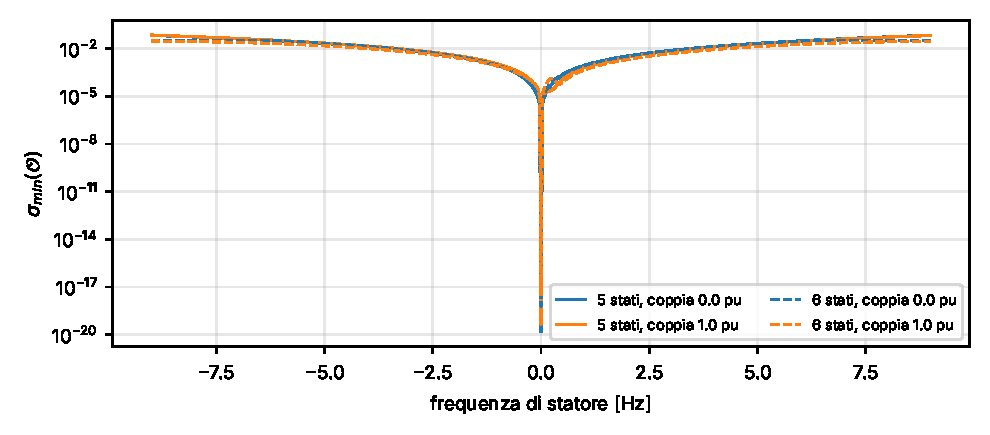
\includegraphics[width=0.85\linewidth]{figures/fig_observability.pdf}
\caption{Minimo valore singolare della matrice di osservabilità del modello linearizzato nel riferimento sincrono, in funzione della frequenza di statore: cinque stati (linea continua) e sei stati (tratteggio), coppia nulla e nominale.}
\label{fig:osservabilita}
\end{figure}

\subsection{Tensione in ingresso, ritardi e tempo morto}
\label{sec:tensione}

L'EKF integra la tensione: ogni errore sulla tensione in ingresso diventa un errore di stima, e a bassa velocità, dove la forza controelettromotrice è piccola, l'effetto relativo è grande. Tre aspetti vanno curati.

\emph{Scala}. La modulazione dei modelli (guadagno $\sqrt3/2$ seguito da \code{sv\_pwm\_process}, che ha come unità $\tfrac23 u_{dc}$) dà $u = u_{dc}/\sqrt3$ per unità di tensione di controllo. In pu di macchina la tensione è quindi $u_{ctrl}\,u_{dc}/(\sqrt3\,u_b)$, con la $u_{dc}$ misurata: \num{1.845}\,$u_{ctrl}$ a \SI{1200}{V}.

\emph{Tempo}. La tensione calcolata al passo $k$ è applicata nell'intervallo $[k+1, k+2]$. L'EKF al passo $k+1$ deve ricevere la tensione applicata in $[k, k+1]$, cioè quella calcolata al passo $k-1$: un ritardo unitario sulla tensione di uscita del regolatore, espressa nel riferimento stazionario con l'angolo anticipato con cui è stata applicata.

\emph{Tempo morto}. L'errore medio di tensione per fase è $\Delta v = t_d f_{pwm} u_{dc} = \SI{3}{\micro s}\cdot\SI{4}{kHz}\cdot\SI{1200}{V} = \SI{14.4}{V}$, con il segno opposto alla corrente di fase \cite{pwrdeadtime}. Come vettore vale $\tfrac43\Delta v = \SI{19.2}{V}$, \num{0.051} pu: nove volte la caduta resistiva totale alla corrente nominale e quanto la forza controelettromotrice al \SI{5}{\percent} della velocità. Va compensato in avanti sulla modulazione con il segno delle correnti di riferimento, $\Delta v\,\mathrm{sat}(i_{k,ref}/I_{band})$ per fase con una banda stretta ($I_{band} = \SI{10}{A}$), e l'EKF deve ricevere la tensione del regolatore senza la compensazione, che rappresenta la tensione realmente applicata. La banda va adattata all'ondulazione di corrente e alle capacità dei dispositivi, che a bassa velocità sono di pochi ampere. Quanto deve essere precisa la compensazione lo dicono le prove della Sez.~\ref{sec:sensibilita}: a coppia nominale e \SI{5}{\percent} di velocità serve un errore d'ampiezza entro circa \SI{10}{\percent}. Se non lo si ottiene, la caratteristica dell'inverter si identifica alla messa in servizio \cite{holtz2002b}, oppure si stima in linea l'ampiezza dell'errore di tensione con uno stato aggiuntivo del filtro (Sez.~\ref{sec:aperti}).

% =====================================================================================================
\section{Prove in simulazione}
\label{sec:prove}

\subsection{Modello di simulazione}
\label{sec:modellosim}

Lo script simula la macchina \eqref{eq:corrente}--\eqref{eq:meccanica} in unità fisiche con l'induttore di uscita (Runge-Kutta del quarto ordine, quattro sotto-passi per periodo di controllo) e il controllo discreto a \SI{8}{kHz}: inverter mediato con ritardo di un periodo più la tenuta, angolo anticipato di $1.5\,\ts\,\omega_\psi$, misura delle correnti di fase con rumore e quantizzazione a \SI{12}{bit}, errore di tempo morto $-\Delta v\,\mathrm{sign}(i)$ per fase e compensazione in avanti. Il controllo è quello della Sez.~\ref{sec:foc} con i guadagni proposti, rampa di velocità filtrata da un secondo ordine a \SI{10}{Hz}, limite di coppia \num{1.35} pu e magnetizzazione con $i_{sx} \le \num{0.8}$ pu nel primo secondo. L'EKF è quello della Sez.~\ref{sec:ekf} con i parametri nominali; nelle prove con errori di parametro cambiano solo quelli della macchina simulata. Il modello mediato non riproduce l'ondulazione di corrente né la dipendenza del tempo morto dalla corrente vicino allo zero: serve a leggere i meccanismi e gli ordini di grandezza, non sostituisce la simulazione Simulink a interruttori.

Il carico è l'attrito viscoso del modello (\num{0.63} pu di $T_b$ alla velocità sincrona) più una coppia esterna attiva. La coppia nominale vale \num{0.84} pu; con l'attrito, \num{0.2} pu esterni alla velocità nominale danno \num{0.83} pu.

\subsection{R1: stimatori in anello aperto con controllo a encoder}
\label{sec:r1}

Il controllo usa l'encoder; sugli stessi dati girano in anello aperto l'EKF proposto con la predizione al secondo ordine, lo stesso con Eulero e l'EKF della libreria. Profilo: magnetizzazione per \SI{1}{s}, rampa alla velocità nominale in \SI{1}{s}, coppia esterna \num{0.2} pu a \SI{2.5}{s} (Fig.~\ref{fig:r1}). A velocità e coppia nominali:
\begin{itemize}
\item EKF proposto, secondo ordine: errore d'angolo \SI{-0.07}{\degree}, errore di velocità \num{-0.0004} pu, coppia di carico stimata \num{0.828} pu contro \num{0.828} reale;
\item stesso EKF con Eulero: errore d'angolo \SI{-18.35}{\degree}, errore di velocità \num{-0.0349} pu: è l'effetto della \eqref{eq:wcrit};
\item EKF della libreria, con la tensione nella scala corretta: \SI{4.61}{\degree} di angolo, \num{-0.0132} pu di velocità e modulo del flusso stimato \num{1.162} pu contro \num{1.004} reale; con la scala di tensione di inv\_im (Sez.~\ref{sec:libreria}, fattore \num{0.770}): \SI{2.23}{\degree}, \num{-0.0160} pu, flusso \num{0.872} pu.
\end{itemize}
L'EKF della libreria segue la velocità perché la sua covarianza sulla velocità è grande (la velocità vi si comporta come una passeggiata aleatoria rapida) e assorbe gli errori di modello nel modulo del flusso: con la tensione scalata di \num{0.770} il flusso stimato scende di circa il \SI{25}{\percent}. Nel controllo senza sensore l'anello di flusso porterebbe a 1 il flusso stimato, cioè il flusso vero a circa \num{0.86} pu con la scala corretta e a \num{1.15} pu con quella di inv\_im.

\begin{figure}[htb]
\centering
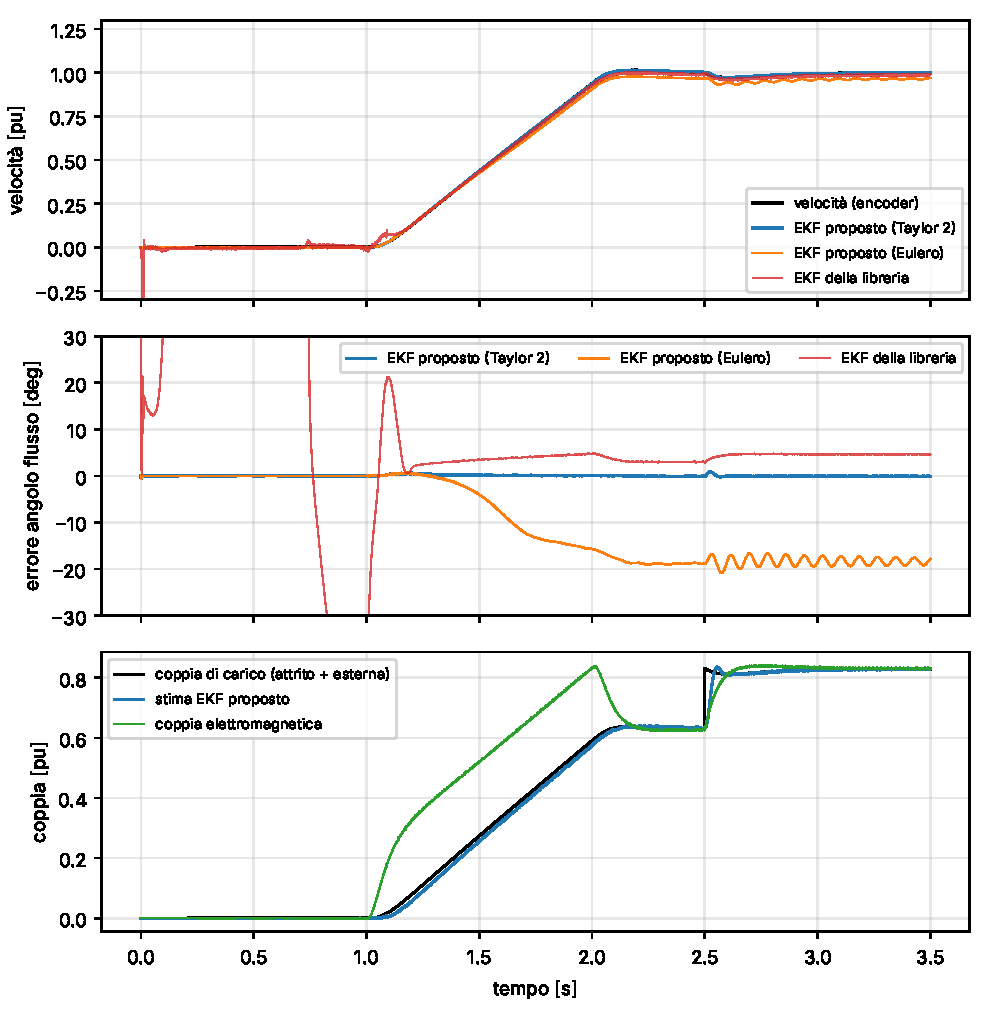
\includegraphics[width=0.85\linewidth]{figures/fig_ekf_openloop.pdf}
\caption{R1: controllo con encoder, stimatori in anello aperto. Velocità, errore sull'angolo del flusso rotorico, coppia di carico (attrito più coppia esterna) e sua stima.}
\label{fig:r1}
\end{figure}

\subsection{R2: controllo senza sensore con parametri nominali}
\label{sec:r2}

L'EKF proposto chiude l'anello: angolo, flusso e velocità del controllo vengono dal filtro. Profilo: magnetizzazione, rampa alla velocità nominale, coppia nominale, rampa fino al \SI{5}{\percent} della velocità e, da \SI{5.5}{s}, coppia esterna portata da \num{0.2} a \num{0.8} pu in \SI{1}{s} (coppia nominale al \SI{5}{\percent}) (Fig.~\ref{fig:r2}). Gli errori a regime restano piccoli in tutto il campo:
\begin{itemize}
\item velocità e coppia nominali: errore di velocità \num{-0.0004} pu, errore d'angolo \SI{-0.07}{\degree}, corrente \SI{400}{A} efficaci;
\item \SI{5}{\percent} con \num{0.23} pu: errore di velocità meno di \num{1e-4} pu, errore d'angolo \SI{0.01}{\degree};
\item \SI{5}{\percent} con coppia nominale: errore di velocità \num{-0.0001} pu, errore d'angolo \SI{-0.15}{\degree}, corrente \SI{403}{A} efficaci.
\end{itemize}
L'errore massimo di velocità, \num{0.0079} pu, è al gradino di carico alla velocità nominale; l'errore d'angolo non supera \SI{1.2}{\degree} dopo la partenza.

\begin{figure}[htb]
\centering
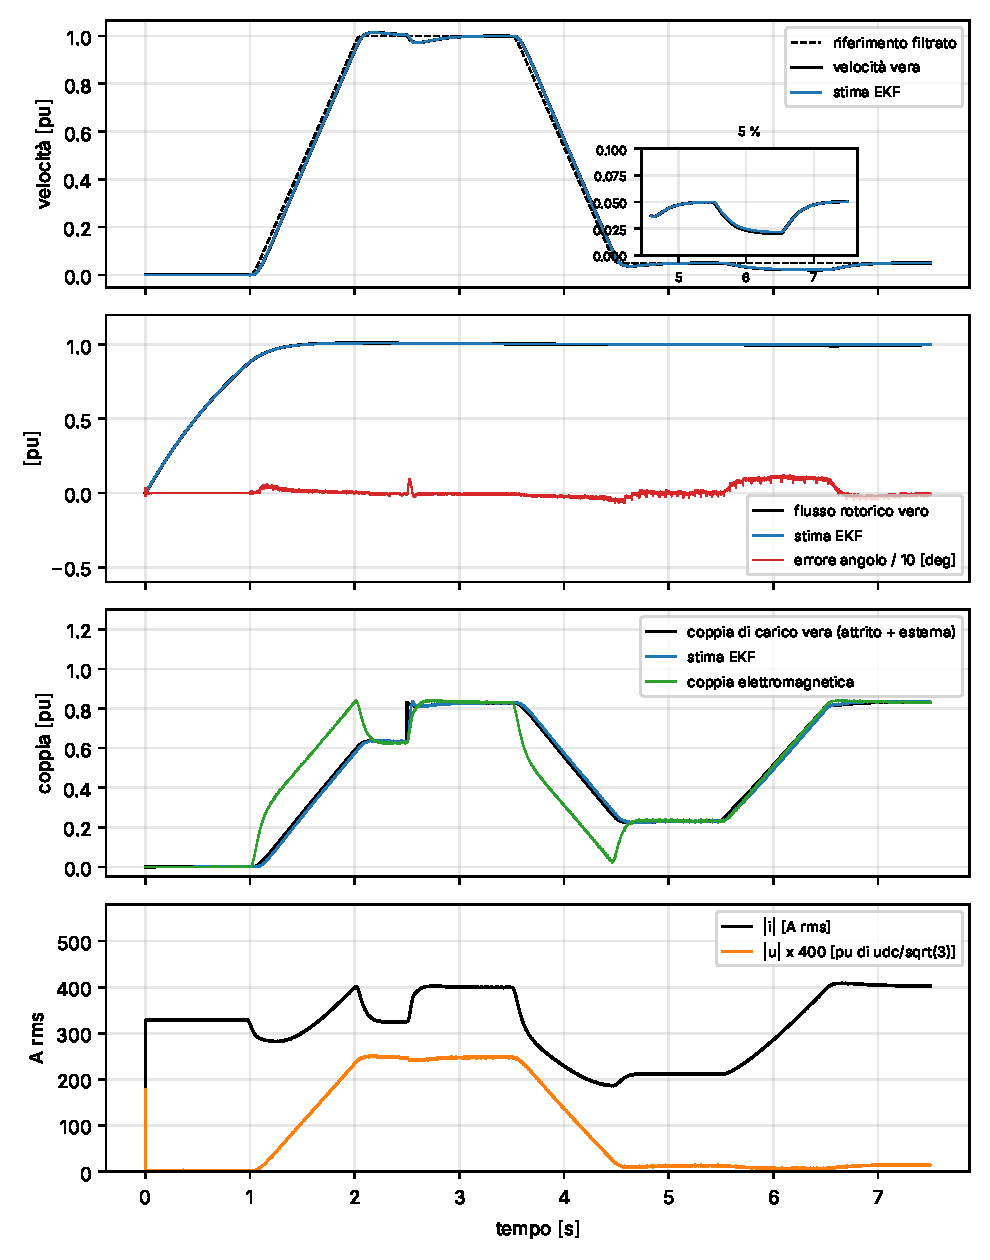
\includegraphics[width=0.85\linewidth]{figures/fig_sensorless_run.pdf}
\caption{R2: controllo senza sensore con l'EKF proposto e parametri nominali. Velocità (riferimento, vera e stimata, con dettaglio al \SI{5}{\percent}), flusso rotorico vero e stimato con l'errore d'angolo, coppia di carico e sua stima, corrente e tensione.}
\label{fig:r2}
\end{figure}

\emph{Senza compensazione del tempo morto} (R2b) alla velocità nominale l'errore d'angolo è ancora piccolo (\SI{-0.91}{\degree}), ma al \SI{5}{\percent} la stima diverge già con \num{0.23} pu: il flusso stimato sale a \num{3.4} pu, la velocità stimata resta vicina al riferimento mentre quella vera scende a \num{-0.17} pu e, con la coppia nominale, la macchina è trascinata indietro dal carico. È il caso tipico di perdita della macchina a bassa velocità.

\subsection{R3: errori di parametro e compensazione imperfetta}
\label{sec:r3}

Le resistenze di statore e di rotore della macchina sono il \SI{30}{\percent} più alte di quelle del modello (macchina calda) e la compensazione del tempo morto vale il \SI{90}{\percent} (R3) o l'\SI{80}{\percent} (R3b) dell'errore vero (Fig.~\ref{fig:r3}). Alla velocità nominale le due prove sono uguali (errore di velocità \num{0.0008} pu, angolo \SI{-0.17}{\degree}). Al \SI{5}{\percent} con \num{0.23} pu R3 ha \SI{-2.6}{\degree} di errore d'angolo e \num{0.0021} pu di errore di velocità; con la coppia nominale \SI{-0.21}{\degree} e \num{0.0032} pu, con flusso vero \num{0.948} pu. R3b invece perde la macchina durante la rampa di carico al \SI{5}{\percent}: l'errore residuo di tensione (\SI{20}{\percent} di \SI{14.4}{V}, circa \SI{2.9}{V} per fase) sposta la stima di velocità verso l'alto, l'anello di velocità rallenta la macchina vera, la frequenza di statore si avvicina a zero e il filtro perde osservabilità.

\begin{figure}[htb]
\centering
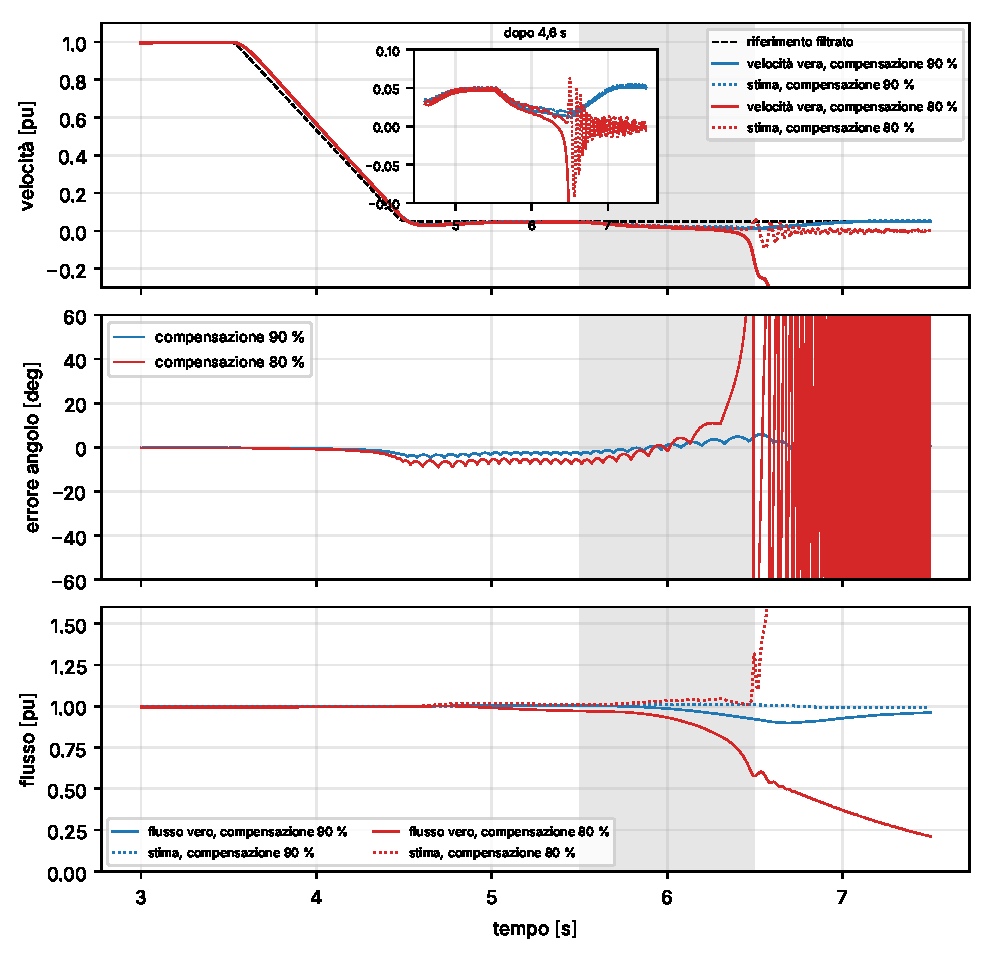
\includegraphics[width=0.85\linewidth]{figures/fig_sensitivity.pdf}
\caption{R3: resistenze di statore e di rotore della macchina +\SI{30}{\percent}, compensazione del tempo morto al \SI{90}{\percent} (blu) e all'\SI{80}{\percent} (rosso). Velocità vera e stimata, errore d'angolo, flusso vero e stimato; in grigio la rampa di carico al \SI{5}{\percent}.}
\label{fig:r3}
\end{figure}

\subsection{R4: inversione lenta attraverso la velocità nulla}
\label{sec:r4}

Con una coppia esterna attiva di \num{0.2} pu il riferimento passa da $+\SI{5}{\percent}$ a $-\SI{5}{\percent}$ in \SI{2}{s}; la frequenza di statore attraversa lo zero intorno a \SI{3.5}{s} e da lì la macchina rigenera (Fig.~\ref{fig:r4}). Con i parametri nominali l'attraversamento costa un errore d'angolo massimo di \SI{17.7}{\degree} e a $-\SI{5}{\percent}$ resta un errore di \SI{4.5}{\degree} con il flusso vero a \num{0.925} pu. Senza tempo morto, oppure con la banda della compensazione ridotta a \SI{3}{A} (aderente al segno ideale dell'errore nel modello mediato), lo stesso profilo dà al massimo \SI{2.9}{\degree} e \SI{3.2}{\degree} in tutto il transitorio, e meno di \SI{0.1}{\degree} a $-\SI{5}{\percent}$: l'errore viene dalla forma della compensazione vicino agli zeri delle correnti di fase, che in rigenerazione a bassa velocità pesa di più. Nel convertitore reale la forma giusta è quella della caratteristica misurata dell'inverter \cite{holtz2002b}. Con gli errori di R3 (compensazione al \SI{90}{\percent}) l'errore d'angolo arriva a \SI{34}{\degree} e a $-\SI{5}{\percent}$ vale \SI{9.7}{\degree}. L'attraversamento lento sotto carico è quindi il caso limite del sistema: si fa, ma con margini piccoli.

\begin{figure}[htb]
\centering
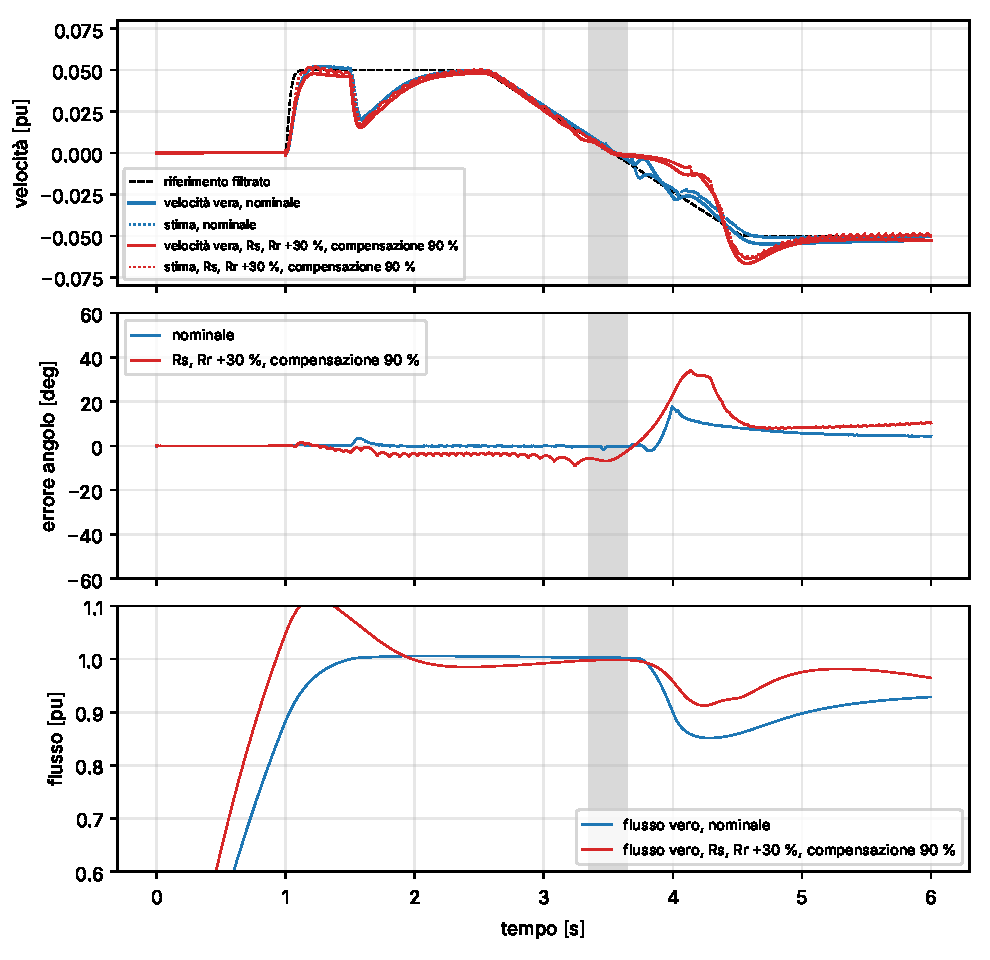
\includegraphics[width=0.85\linewidth]{figures/fig_reversal.pdf}
\caption{R4: inversione lenta da $+\SI{5}{\percent}$ a $-\SI{5}{\percent}$ con coppia attiva di \num{0.2} pu, parametri nominali (blu) e con gli errori di R3 (rosso). In grigio l'intervallo in cui la frequenza di statore attraversa lo zero.}
\label{fig:r4}
\end{figure}

\subsection{Sensibilità al 5\,\% della velocità}
\label{sec:sensibilita}

La Tab.~\ref{tab:sensibilita} riporta errore di velocità ed errore d'angolo al \SI{5}{\percent} della velocità con un solo errore per volta: magnetizzazione, \SI{5}{\percent} di velocità, \num{0.2} pu di coppia esterna (\num{0.23} pu con l'attrito) e poi rampa fino alla coppia nominale.

\begin{table}[H]
\centering\small
\begin{tabular}{@{}lcccc@{}}
\toprule
 & \multicolumn{2}{c}{Coppia \num{0.23} pu} & \multicolumn{2}{c}{Coppia nominale \num{0.83} pu} \\
\cmidrule(lr){2-3}\cmidrule(lr){4-5}
Errore & velocità [pu] & angolo [\si{\degree}] & velocità [pu] & angolo [\si{\degree}] \\
\midrule
nominale & \num{0.0000} & \num{-0.05} & \num{-0.0001} & \num{-0.06} \\
compensazione del tempo morto all'\SI{85}{\percent} & \num{0.0019} & \num{-4.29} & \num{0.0026} & \num{0.05} \\
compensazione al \SI{90}{\percent} & \num{0.0014} & \num{-2.58} & \num{0.0022} & \num{0.84} \\
compensazione al \SI{110}{\percent} & \num{-0.0031} & \num{-0.35} & \num{-0.0025} & \num{-1.43} \\
compensazione al \SI{115}{\percent} & \num{-0.0063} & \num{-3.87} & \multicolumn{2}{c}{perso (macchina ferma, flusso \num{1.50} pu)} \\
banda della compensazione \SI{29}{A} & \num{0.0000} & \num{-0.06} & \num{0.0000} & \num{0.09} \\
$R_s$ $+\SI{30}{\percent}$ & \num{0.0002} & \num{-0.19} & \num{0.0004} & \num{0.26} \\
$R_s$ $-\SI{30}{\percent}$ & \num{-0.0002} & \num{0.10} & \num{-0.0005} & \num{-0.31} \\
$R_r$ $+\SI{30}{\percent}$ & \num{0.0004} & \num{0.20} & \num{0.0010} & \num{0.01} \\
$R_r$ $-\SI{30}{\percent}$ & \num{-0.0028} & \num{-3.90} & \num{-0.0012} & \num{-0.28} \\
$L_m$ $-\SI{10}{\percent}$ & \num{-0.0036} & \num{-6.10} & \num{-0.0015} & \num{-2.53} \\
$L_m$ $+\SI{10}{\percent}$ & \num{0.0016} & \num{2.35} & \num{0.0014} & \num{2.31} \\
\bottomrule
\end{tabular}
\caption{Sensibilità al \SI{5}{\percent} della velocità: errore della stima di velocità ed errore sull'angolo del flusso a regime, un errore per volta. ``perso'' indica che la stima diverge e il carico trascina la macchina.}
\label{tab:sensibilita}
\end{table}

Le resistenze pesano poco: con il \SI{30}{\percent} di errore su $R_s$ l'angolo resta entro \SI{0.31}{\degree}, su $R_r$ entro \SI{0.20}{\degree} con $R_r$ più alta e \SI{3.9}{\degree} con $R_r$ più bassa a coppia ridotta. Un errore del \SI{30}{\percent} su $R_s$ vale \num{0.0009} pu, un decimo della resistenza $\Rp$ vista dall'inverter, e alla corrente nominale sposta la tensione di \num{0.0009} pu contro \num{0.05} pu di forza controelettromotrice al \SI{5}{\percent}. Il residuo del tempo morto con la compensazione all'\SI{85}{\percent} vale invece $\num{0.15}\cdot\num{0.051} = \num{0.0077}$ pu, otto volte di più. Pesano quindi soprattutto il tempo morto e $L_m$ (saturazione: \SI{10}{\percent} di errore danno fino a \SI{6.1}{\degree}). L'ampiezza della compensazione deve stare fra l'\SI{85}{\percent} e il \SI{110}{\percent} dell'errore vero, cioè entro circa \SI{2}{V} per fase su \SI{14.4}{V}: al \SI{115}{\percent} il controllo si blocca con la macchina ferma e il flusso a \num{1.5} pu, all'\SI{80}{\percent} con le resistenze calde perde la macchina (R3b). Una banda della compensazione più larga (\SI{29}{A} invece di \SI{10}{A}) non cambia il funzionamento in motore; in rigenerazione la forma della compensazione vicino agli zeri delle correnti conta di più (Sez.~\ref{sec:r4}).

\clearpage
% =====================================================================================================
\section{Revisione dell'EKF della libreria}
\label{sec:libreria}

L'EKF di inv\_im è il blocco \code{ekf/extended\_kalman\_observer} di \code{inv\_im\_param.slx}, configurato da \code{ekf\_im\_setup} con $\alpha$, $\beta$, $\gamma$, $\sigma$, $\mu$, $L_m$, $J_{m,norm}$ e $\ts$ di \code{im\_setup}. Lo stato è lo stesso della Sez.~\ref{sec:stato}; la Jacobiana è scritta come $A(x) = A_1 + A_2 x_1 + A_3 x_2 + A_4 x_3 + A_5 x_4 + A_6 x_5$ e la predizione come $\xh_{k+1|k} = A_d(\xh_k)\,\xh_k + \ts\wb B u_k$. La Tab.~\ref{tab:libreria} riassume le differenze rispetto al modello corretto; le prime cinque sono errori, le altre scelte da rivedere.

\begin{table}[H]
\centering\small
\begin{tabular}{@{}R{0.6cm}R{6.6cm}R{8.3cm}@{}}
\toprule
& \textbf{Implementazione della libreria} & \textbf{Effetto e correzione} \\
\midrule
1 & Riga meccanica con $\mu = L_m/(J_{m,norm}L_r)$ e $1/J_{m,norm}$, moltiplicata per $\ts\wb$; $J_{m,norm} = \tfrac12 J\omega_{mb}/T_{nom} = \SI{0.1437}{s}$ & Nel tempo normalizzato il coefficiente corretto è $\kr/(\taum\wb)$ con $\taum = J\omega_{mb}/T_b = \SI{0.2411}{s}$: il guadagno della coppia è $\taum\wb/J_{m,norm} = \num{632}$ volte troppo alto, quello di $T_L$ anche. Usare $\taum$ in secondi senza $\wb$, con la base di coppia $T_b$ \\
2 & Predizione $A_d(\xh)\,\xh$, cioè Jacobiana per stato & I termini bilineari ($\omega\psi$, $\psi i$) compaiono due volte. Nelle righe elettriche il termine $A_6 x_5$ è scalato per $\ts$ invece che per $\ts\wb$, quindi la seconda copia vale $1/\wb$ della prima e l'errore è dello \SI{0.27}{\percent}; nella riga meccanica la coppia è raddoppiata (con il punto 1: \num{1265} volte). Usare $\xh + \ts f(\xh,u)$ con la \eqref{eq:f} \\
3 & Predizione e covarianza con Eulero in avanti & Modo del flusso instabile sopra \num{0.28} pu (Sez.~\ref{sec:discretizzazione}). Usare la \eqref{eq:taylor2} \\
4 & $\sigma$ e $R_s$ della sola macchina & L'induttore di uscita di inv\_im porta $\sigma$ da \num{0.172} a \num{0.306} (\num{1.78} volte) e $R_s$ da \num{0.0031} a \num{0.0059}: usare $\sigma_t$, $R_{s,t}$ e i $\beta$, $\gamma$ corrispondenti \\
5 & Tensione $u_{ctrl}\cdot$\code{u\_im\_scale\_ekf} $= u_{ctrl}\,(2/3)^2 u_{dc,nom}/u_b$ & La modulazione dà $u_{dc}/\sqrt3$ per unità di controllo: la tensione data al filtro è $(2/3)^2\sqrt3 = \num{0.770}$ volte quella vera, e $u_{dc,nom} = \SI{1070}{V}$ (set \SI{690}{V}) contro \SI{1200}{V} della batteria toglie un altro \SI{11}{\percent}. L'EKF del PMSM nello stesso init usa già $\sqrt3/2\cdot2/3 = 1/\sqrt3$. Usare $u_{ctrl}\,u_{dc,mis}/(\sqrt3 u_b)$ \\
6 & $Q = \tfrac{\ts}{10}\mathrm{diag}(\ts^2, \ts^2, \ts, \ts, 1, 1)$, $R = \ts I$ & $R = \num{1.25e-4}$ pu$^2$ (\SI{6.5}{A}) è 40 volte la varianza del rumore modellato; $Q_\omega = Q_{T_L} = \num{1.25e-5}$ per passo fa della velocità una passeggiata aleatoria rapida, che maschera in parte i punti 1 e 2 e passa rumore alla velocità. Ricavare $Q$ e $R$ da rumore e incertezze (Sez.~\ref{sec:covarianze}) \\
7 & $\xh_0 = [0,0,1,1,0,0]\,\ts$, $P_0 = 0$ & Covarianza iniziale nulla: il filtro parte certo di uno stato sbagliato. Usare $P_0$ diagonale e il blocco durante la magnetizzazione \\
8 & Switch encoder/sensorless con lo \code{Step} \code{time\_use\_im\_ekf} commentato & L'EKF non è mai entrato nell'anello. Prima prova consigliata: in parallelo all'encoder come in R1, poi in anello \\
\bottomrule
\end{tabular}
\caption{EKF della libreria (\code{ekf\_im\_setup}, \code{inv\_im\_param.slx}): differenze rispetto al modello corretto, effetto e correzione.}
\label{tab:libreria}
\end{table}

Con la scala di tensione corretta l'EKF della libreria, in anello aperto a velocità nominale, sbaglia l'angolo di \SI{4.61}{\degree} e la velocità di \num{-0.0132} pu (Sez.~\ref{sec:r1}). Il risultato non è peggiore perché la grande covarianza di processo sulla velocità lo trasforma in un osservatore adattativo ad alto guadagno, che insegue la velocità con le innovazioni di corrente qualunque sia la riga meccanica. Lo stesso meccanismo però scarica gli errori di modello sul modulo del flusso (\num{1.162} pu stimati contro \num{1.004} reali, \num{0.872} pu con la scala di inv\_im), e in un controllo senza sensore l'anello di flusso li trasformerebbe in errori di magnetizzazione reali. Correggere i punti 1--5 e ritarare $Q$ e $R$ porta all'EKF della Sez.~\ref{sec:ekf}.

% =====================================================================================================
\section{Raccomandazioni}
\label{sec:raccomandazioni}

\begin{enumerate}
\item \emph{FOC}: PI di corrente con lo zero sul polo e disaccoppiamento in avanti ($f_c = \SI{200}{Hz}$); anello di flusso con feed-forward, $k_p = 6$, $k_i = k_p/\taur$ e integrale bloccato in saturazione; uscita del PI di velocità come coppia, divisa per $\kr\hat\psi$; magnetizzazione completa prima della rampa; deflussaggio legato alla tensione; feed-forward della $u_{dc}$ misurata.
\item \emph{Modello dell'EKF}: sei stati con la meccanica in $\taum$ e base di coppia $T_b$; parametri con l'induttore di uscita; predizione \eqref{eq:taylor2} (almeno per lo stato); aggiornamento di Joseph.
\item \emph{Tensione}: scala $u_{dc,mis}/(\sqrt3 u_b)$, ritardo di un passo, tensione del regolatore senza la compensazione del tempo morto.
\item \emph{Tempo morto}: compensazione in avanti sul segno delle correnti di riferimento con banda di pochi ampere, ampiezza verificata alla messa in servizio entro circa il \SI{10}{\percent}; a bassa velocità è il requisito più severo di tutto il sistema.
\item \emph{Covarianze}: $R$ dal rumore e dalla quantizzazione; $Q_{T_L}$ come parametro di taratura principale; $P_0$ non nulla; blocco di $\hat\omega$ e $\hat T_L$ durante la magnetizzazione.
\item \emph{Campo di funzionamento}: coppia nominale fino a circa il \SI{5}{\percent} della velocità (\SI{3}{Hz}); sotto, e in rigenerazione a bassa velocità, evitare il funzionamento prolungato vicino alla frequenza di statore nulla; un'inversione sotto carico va fatta rapidamente.
\item \emph{Messa in servizio in inv\_im}: correggere \code{ekf\_im\_setup} e la scala di tensione, provare l'EKF in parallelo all'encoder (come R1), poi chiudere l'anello attivando lo switch.
\end{enumerate}

\section{Punti aperti}
\label{sec:aperti}

\begin{itemize}
\item La scala di tensione e la presenza dell'induttore nel modello della macchina di inv\_im vanno confermate in Simulink confrontando la tensione data al filtro con quella ai morsetti, in pu, a velocità nominale.
\item Le prove sono su un modello mediato con tempo morto ideale: vanno ripetute sul modello a interruttori, dove l'ondulazione di corrente e le capacità dei dispositivi rendono l'errore di tempo morto dipendente dalla corrente.
\item La saturazione magnetica non è modellata: a flusso nominale $L_m$ dipende da $i_{sx}$, e la Tab.~\ref{tab:sensibilita} mostra che \SI{10}{\percent} di errore su $L_m$ costano qualche grado. Una curva $L_m(\psi)$ nel modello del filtro è il passo successivo.
\item Per allargare il margine sul tempo morto si può aggiungere allo stato l'ampiezza dell'errore di tensione o la resistenza di statore \cite{barut2008}, con un'analisi di osservabilità dedicata: a regime e a bassa velocità le due grandezze e la velocità non sono separabili senza variazioni del punto di lavoro.
\item I guadagni proposti vanno riportati nei modelli (blocchi dei PI e struttura dell'anello di flusso, che richiede la modifica del sottosistema) e verificati con le simulazioni Simulink.
\end{itemize}

\end{onehalfspace}

% =====================================================================================================
\appendix
\section{Matrici del filtro}
\label{app:matrici}

Con $x = [i_\alpha, i_\beta, \psi_\alpha, \psi_\beta, \omega, T_L]^T$ e i coefficienti con l'induttore di uscita, la Jacobiana della \eqref{eq:f} è
\begin{equation*}
A(x) =
\begin{bmatrix}
-\wb\gamma & 0 & \wb\beta\alpha & \wb\beta\omega & \wb\beta\psi_\beta & 0\\
0 & -\wb\gamma & -\wb\beta\omega & \wb\beta\alpha & -\wb\beta\psi_\alpha & 0\\
\wb\alpha L_m & 0 & -\wb\alpha & -\wb\omega & -\wb\psi_\beta & 0\\
0 & \wb\alpha L_m & \wb\omega & -\wb\alpha & \wb\psi_\alpha & 0\\
-\kr\psi_\beta/\taum & \kr\psi_\alpha/\taum & \kr i_\beta/\taum & -\kr i_\alpha/\taum & 0 & -1/\taum\\
0 & 0 & 0 & 0 & 0 & 0
\end{bmatrix},
\qquad
C = \begin{bmatrix} 1 & 0 & 0 & 0 & 0 & 0\\ 0 & 1 & 0 & 0 & 0 & 0\end{bmatrix}.
\end{equation*}
Valori per questa macchina e per $\ts = \SI{125}{\micro s}$: $\sigma_t = \num{0.30631}$, $R_{s,t} = \num{0.00589}$, $L_m = \num{2.1956}$, $L_r = \num{2.2833}$, $\kr = \num{0.9616}$, $\alpha = \num{0.001857}$, $\beta_t = \num{3.139}$, $\gamma_t = \num{0.03203}$, $\taum = \SI{0.2411}{s}$, $\wb = \SI{376.99}{rad/s}$; $R = \num{3.03e-6}\,I_2$; $Q = \mathrm{diag}(\num{9.47e-6}, \num{9.47e-6}, \num{e-10}, \num{e-10}, \num{e-10}, \num{e-6})$.

\section{Un passo del filtro in pseudocodice}
\label{app:pseudocodice}

\begin{small}
\begin{verbatim}
% ingressi: x (6x1), P (6x6); u = [ua; ub]: tensione applicata in [k,k+1] (pu di ub);
%           y = [ia; ib]: corrente campionata in k+1 (pu di ib);
%           hold: macchina ferma in magnetizzazione
if hold
    x(5:6) = 0;  P(5:6,:) = 0;  P(:,5:6) = 0;  Qk = Q;  Qk(5:6,5:6) = 0;
else
    Qk = Q;                      % alla prima uscita da hold: P(5,5) = P(6,6) = 1e-4
end
f = [wb*(-g*x(1) + b*a*x(3) + b*x(5)*x(4) + u(1)/s);
     wb*(-g*x(2) + b*a*x(4) - b*x(5)*x(3) + u(2)/s);
     wb*( a*Lm*x(1) - a*x(3) - x(5)*x(4));
     wb*( a*Lm*x(2) - a*x(4) + x(5)*x(3));
     (kr*(x(3)*x(2) - x(4)*x(1)) - x(6))/tm;
     0];
A = jacobiana(x);                % Appendice A
xp = x + ts*f + ts^2/2*(A*f);    % predizione al secondo ordine
F = eye(6) + ts*A;               % covarianza: basta il primo ordine (o + (ts*A)^2/2)
Pp = F*P*F' + Qk;
S = Pp(1:2,1:2) + R;             % 2x2, inversa esplicita
K = Pp(:,1:2)/S;
x = xp + K*(y - xp(1:2));
IKC = eye(6);  IKC(:,1:2) = IKC(:,1:2) - K;
P = IKC*Pp*IKC' + K*R*K';
% uscite: angolo = atan2(x(4), x(3)), modulo del flusso = hypot(x(3), x(4)),
%         velocita' = x(5), coppia di carico = x(6)
\end{verbatim}
\end{small}

% =====================================================================================================
\begin{thebibliography}{99}
\small
\bibitem{blaschke1972} F.~Blaschke, ``The principle of field orientation as applied to the new transvector closed-loop control system for rotating-field machines,'' \emph{Siemens Review}, vol.~34, pp.~217--220, 1972.
\bibitem{novotny1996} D.~W. Novotny and T.~A. Lipo, \emph{Vector Control and Dynamics of AC Drives}. Oxford University Press, 1996.
\bibitem{leonhard2001} W.~Leonhard, \emph{Control of Electrical Drives}, 3rd ed. Springer, 2001.
\bibitem{harnefors1998} L.~Harnefors and H.-P. Nee, ``Model-based current control of AC machines using the internal model control method,'' \emph{IEEE Trans. Ind. Appl.}, vol.~34, no.~1, pp.~133--141, Jan./Feb. 1998.
\bibitem{holtz2002} J.~Holtz, ``Sensorless control of induction motor drives,'' \emph{Proc. IEEE}, vol.~90, no.~8, pp.~1359--1394, Aug. 2002.
\bibitem{vas1998} P.~Vas, \emph{Sensorless Vector and Direct Torque Control}. Oxford University Press, 1998.
\bibitem{schauder1992} C.~Schauder, ``Adaptive speed identification for vector control of induction motors without rotational transducers,'' \emph{IEEE Trans. Ind. Appl.}, vol.~28, no.~5, pp.~1054--1061, Sep./Oct. 1992.
\bibitem{kubota1993} H.~Kubota, K.~Matsuse, and T.~Nakano, ``DSP-based speed adaptive flux observer of induction motor,'' \emph{IEEE Trans. Ind. Appl.}, vol.~29, no.~2, pp.~344--348, Mar./Apr. 1993.
\bibitem{hinkkanen2004} M.~Hinkkanen and J.~Luomi, ``Stabilization of regenerating-mode operation in sensorless induction motor drives by full-order flux observer design,'' \emph{IEEE Trans. Ind. Electron.}, vol.~51, no.~6, pp.~1318--1328, Dec. 2004.
\bibitem{kalman1960} R.~E. Kalman, ``A new approach to linear filtering and prediction problems,'' \emph{Trans. ASME J. Basic Eng.}, vol.~82, pp.~35--45, 1960.
\bibitem{simon2006} D.~Simon, \emph{Optimal State Estimation: Kalman, $H_\infty$, and Nonlinear Approaches}. Wiley, 2006.
\bibitem{kim1994} Y.-R. Kim, S.-K. Sul, and M.-H. Park, ``Speed sensorless vector control of induction motor using extended Kalman filter,'' \emph{IEEE Trans. Ind. Appl.}, vol.~30, no.~5, pp.~1225--1233, Sep./Oct. 1994.
\bibitem{barut2007} M.~Barut, S.~Bogosyan, and M.~Gokasan, ``Speed-sensorless estimation for induction motors using extended Kalman filters,'' \emph{IEEE Trans. Ind. Electron.}, vol.~54, no.~1, pp.~272--280, Feb. 2007.
\bibitem{barut2008} M.~Barut, S.~Bogosyan, and M.~Gokasan, ``Experimental evaluation of braided EKF for sensorless control of induction motors,'' \emph{IEEE Trans. Ind. Electron.}, vol.~55, no.~2, pp.~620--632, Feb. 2008.
\bibitem{ibarra2004} S.~Ibarra-Rojas, J.~Moreno, and G.~Espinosa-Pérez, ``Global observability analysis of sensorless induction motors,'' \emph{Automatica}, vol.~40, no.~6, pp.~1079--1085, 2004.
\bibitem{holtz2002b} J.~Holtz and J.~Quan, ``Sensorless vector control of induction motors at very low speed using a nonlinear inverter model and parameter identification,'' \emph{IEEE Trans. Ind. Appl.}, vol.~38, no.~4, pp.~1087--1095, Jul./Aug. 2002.
\bibitem{pwrdeadtime} pwr-control, \emph{Dead time in voltage source converters}, nota \path{research/power_electronics/dead_time} del repository repositories-documentation.
\bibitem{pwrgfm} pwr-control, \emph{Grid-forming control in the synchronous dq frame: structure, continuous-time design and discrete implementation}, nota \path{research/power_electronics/grid_forming_control} del repository repositories-documentation, 2026.
\end{thebibliography}

\end{document}
